\documentclass[a4paper,12pt]{article}
\usepackage[utf8]{inputenc}
\usepackage{graphicx}
\usepackage{subcaption}
\usepackage{amsmath}
\usepackage{url}
\usepackage{float}
\usepackage{babel}
\renewcommand{\figurename}{Slika}  % Change "Figure" to "Slika"
\renewcommand{\tablename}{Tabela}

\begin{document}

\begin{titlepage}
    \centering
	\begin{figure}[htbp]
    	\centering
    	
\includegraphics[width=0.4\textwidth]{./logo.png}
	\end{figure}
    { Univerzitet u Beogradu \\ Matematički fakultet\par}
	
    \vfill

    {\Large \textbf{Seminarski rad}\par}

    \vspace{1cm}

    {\Large \textbf{Ocenjivanje broja ljudi na javnom skupu}\par}

    \vfill

    
	
	
	\begin{tabbing}
	\hspace{10cm} \= \hspace{10cm} \= \kill
	\textbf{Mentor:} \>  \textbf{Studenti:} \\
	dr Marija Cuparić \> Lana Matić 143/2021 \\
	Luka Perović \> Anja Milutinović 235/2021 \\
	\> Smer: Informatika
	\end{tabbing}

    \vfill

    \textbf{Datum:} 2024/25

\end{titlepage}
\newpage
\tableofcontents
\newpage
\section{Uvod}

Ocenjivanje broja ljudi na javnim skupovima važno je za bezbednost, logistiku, planiranje resursa i evaluaciju događaja. Tradicionalne metode brojanja na terenu često su skupe, spore i podložne greškama, naročito kada je gužva neujednačena i kada uslovi posmatranja variraju između lokacija.
Cilj ovog rada je procena ukupnog broja ljudi prisutnih na Slaviji 15.3.2025. , na osnovu slika dobijenih iz drona. 
\newline
\newline
\noindent Koristićemo stratifikovano uzorkovanje nad slikama podeljenim mrežom sa automatskim razvrstavanjem ćelija u stratume po gustini, kako bi se efikasno i transparentno ocenili ukupan broj prisutnih ljudi.
Polazni skup podataka čine fotografije dobijene izdvajenjem frejmova iz video-snimka dronom, dalje isečenih u sedam međusobno disjunktnih slika koje pokrivaju različite ulice posmatranog područja.
Koristimo stratifikovano uzorkovanje sa pilot fazom i Neymanov metod raspodele obima uzorka po stratumima.
\newline
\newline
\noindent Rezultati su primenljivi u realnim uslovima i lako se prilagođavaju drugim lokacijama, rezolucijama i opterećenjima scene.
\paragraph{Napomena}
Metod ima ograničenja, jer tačnost zavisi od kvaliteta ulaznih snimaka (osvetljenje, senke, refleksije, zaklanjanja), kao i od stabilnosti veze između vizuelnih signala i stvarne prisutnosti ljudi. Dodatno ograničenje je to što se u ovom pristupu prebrojavaju samo upaljeni blicevi, dok je stvarni broj ljudi sigurno veći od broja registrovanih bliceva.




\newpage
\section{Prikupljanje materijala}

Materijali korišćeni u radu prikupljeni su pomoću snimka dobijenog iz drona \cite{drone_video}, izdvajanjem određenih frejmova koji odgovaraju različitim ulicama. Slike su zatim dodatno isečene tako da nema značajnih preklapanja, radi izbegavanja pojavljivanja istih delova na različitim slikama.
Na narednim slikama prikazani su frejmovi izdvojeni iz snimka dronom.

\begin{figure}[H] 
	\centering 
	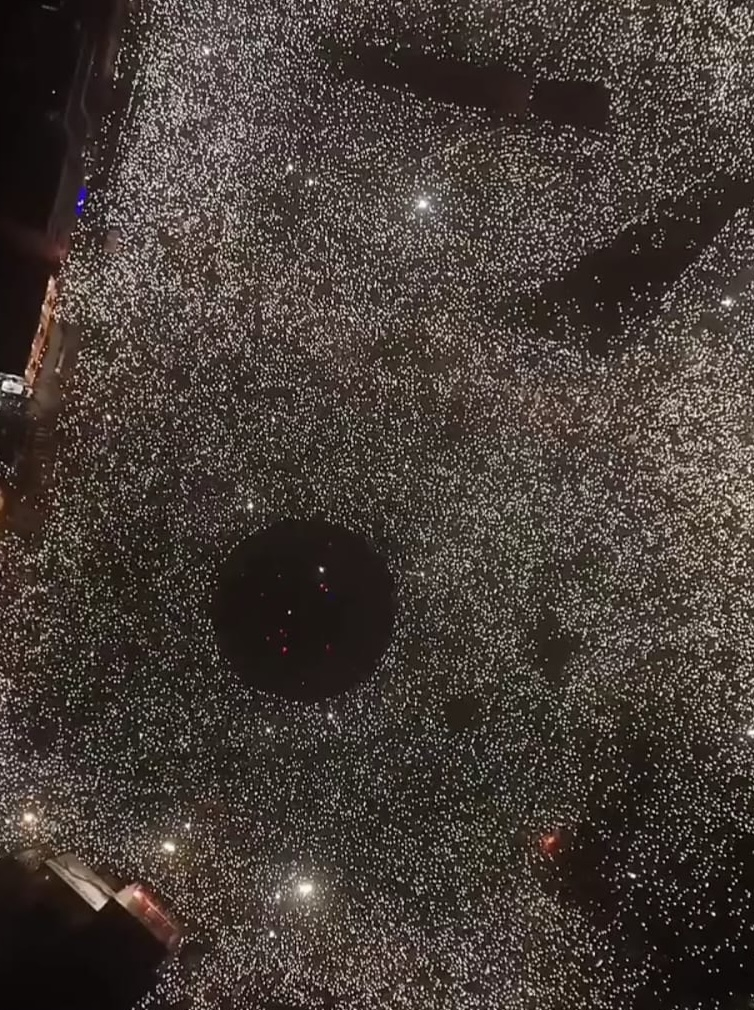
\includegraphics[width=0.8\textwidth]{../images/slavija-centar.jpeg} 
	\caption{Slavija.} 
	\label{fig:slavija} 
\end{figure}

\begin{figure}[H]
	\centering
  
	% Prvi red
	\begin{subfigure}[b]{0.3\textwidth}
	  \centering
	  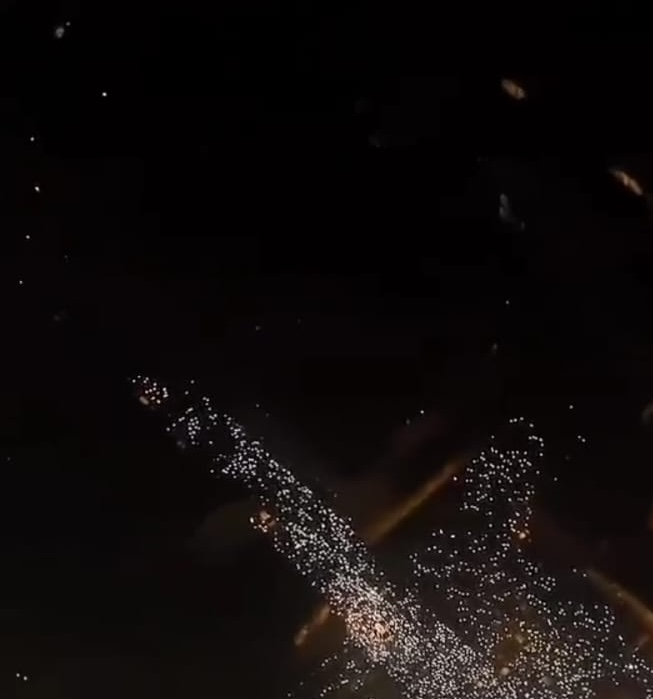
\includegraphics[width=\textwidth]{../images/prote-mateje.jpeg}
	  \caption{Prote Mateje}
	  \label{fig:prote-mateje}
	\end{subfigure}
	\hfill
	\begin{subfigure}[b]{0.3\textwidth}
	  \centering
	  
\includegraphics[width=\textwidth]{../images/nemanjina.jpeg}
	  \caption{Nemanjina}
	  \label{fig:nemanjina}
	\end{subfigure}
	\hfill
	\begin{subfigure}[b]{0.3\textwidth}
		\centering
		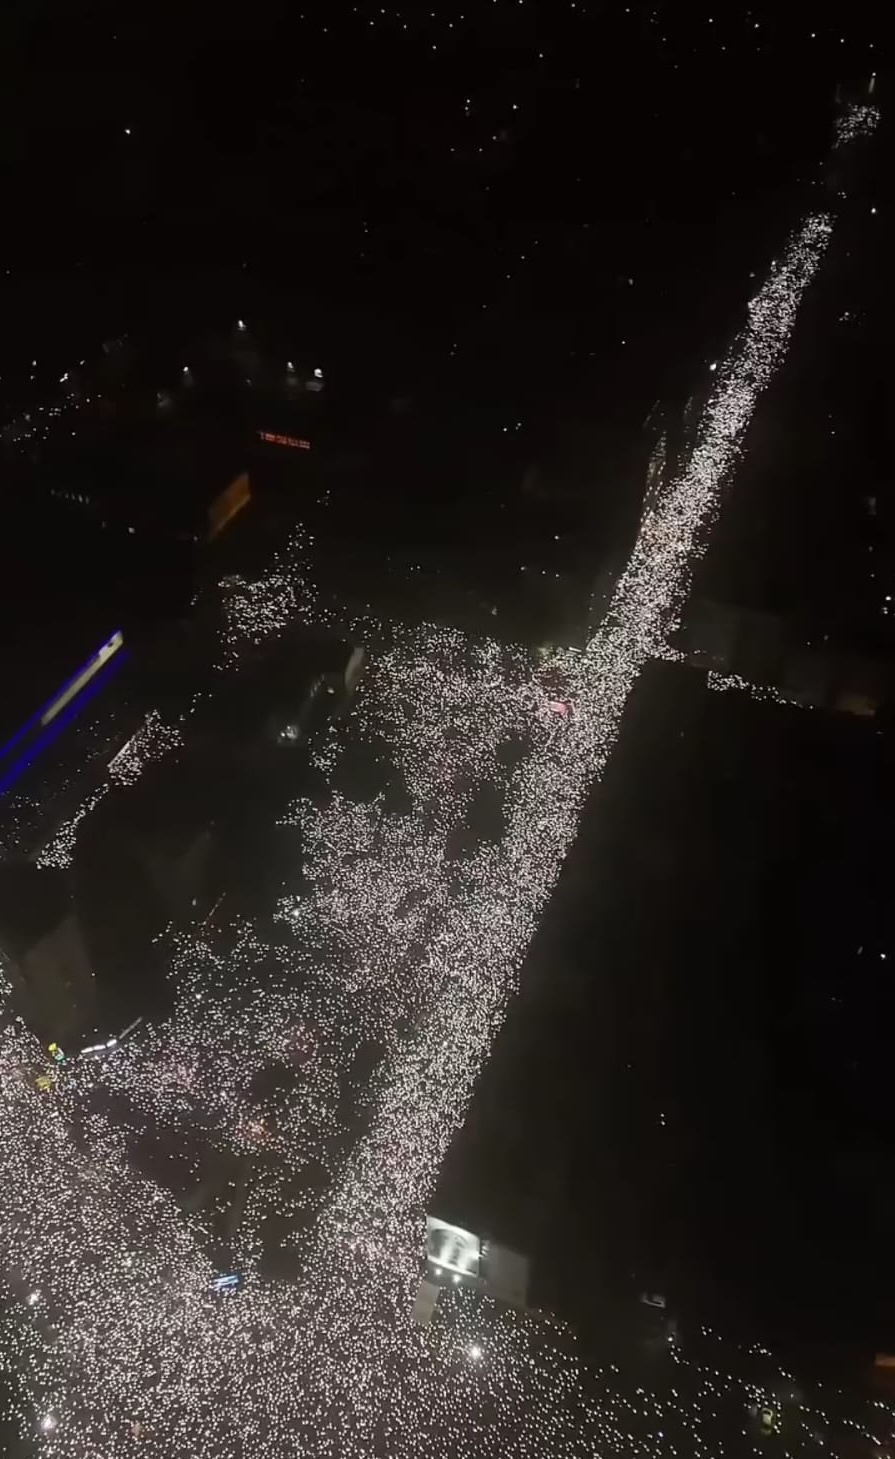
\includegraphics[width=\textwidth]{../images/beogradska.jpeg}
		\caption{Beogradska}
		\label{fig:beogradska}
	\end{subfigure}
  
	\vspace{0.3cm} % razmak između redova
  
	% Drugi red
	\begin{subfigure}[b]{0.3\textwidth}
	  \centering
	  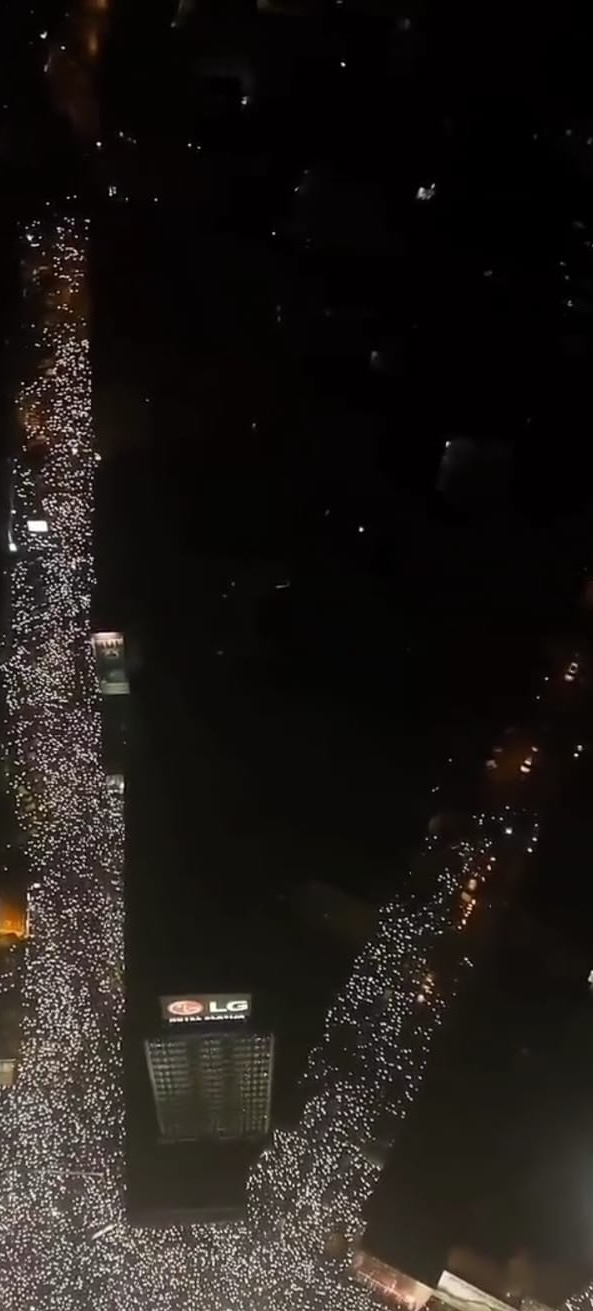
\includegraphics[width=\textwidth]{../images/makenzijeva.jpeg}
	  \caption{Makenzijeva}
	  \label{fig:makenzijeva}
	\end{subfigure}
	\hfill
	\begin{subfigure}[b]{0.3\textwidth}
	  \centering
	  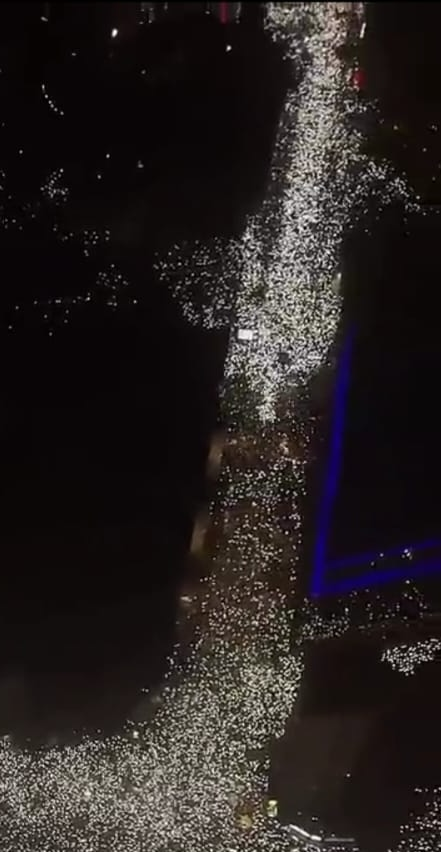
\includegraphics[width=\textwidth]{../images/kralja-milana.jpeg}
	  \caption{Kralja Milana}
	  \label{fig:kralja-milana}
	\end{subfigure}
	\hfill
	\begin{subfigure}[b]{0.3\textwidth}
	  \centering
	  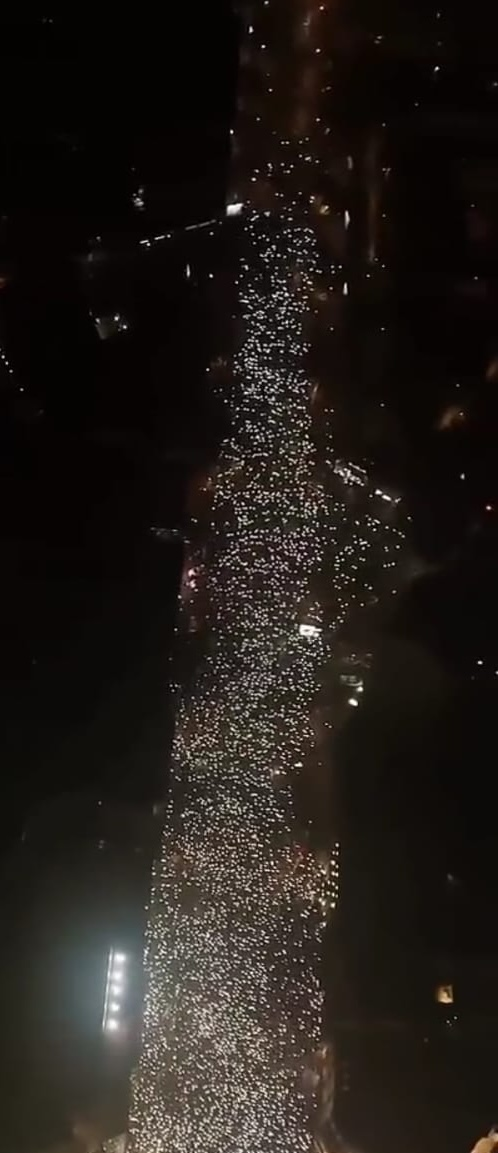
\includegraphics[width=\textwidth]{../images/bulevar-oslobodjenja.jpeg}
	  \caption{Bulevar oslobođenja}
	  \label{fig:bulevar-oslobodjenja}
	\end{subfigure}
  
	\caption{Pregled ulica sa snimka dronom}
\end{figure}

\newpage
\section{Grid i stratifikacija}

Kako bi se omogućili uzorkovanje, svaka ulazna slika je podeljena na pravougaoni grid dimenzija 40 x 40 ćelija. 
Mreža je napravljena u R-u, i za svaku ćeliju su čuvani sledeći atributi: 
jedinstveni identifikator - \texttt{cell\_id}, red i kolonu, koordinate u pikselima \texttt{(x0, x1, y0, y1)}, oznaku zone - \texttt{zone\_id}, 
logičku oznaku - \texttt{include} - da li je ćelija uključena u uzorkovanje i stratumski indeks - stratum.
Informacije čuvamo u tabeli \texttt{strata\_map.csv}, koju zatim popunjavamo.

\begin{figure}[H] 
	\centering 
	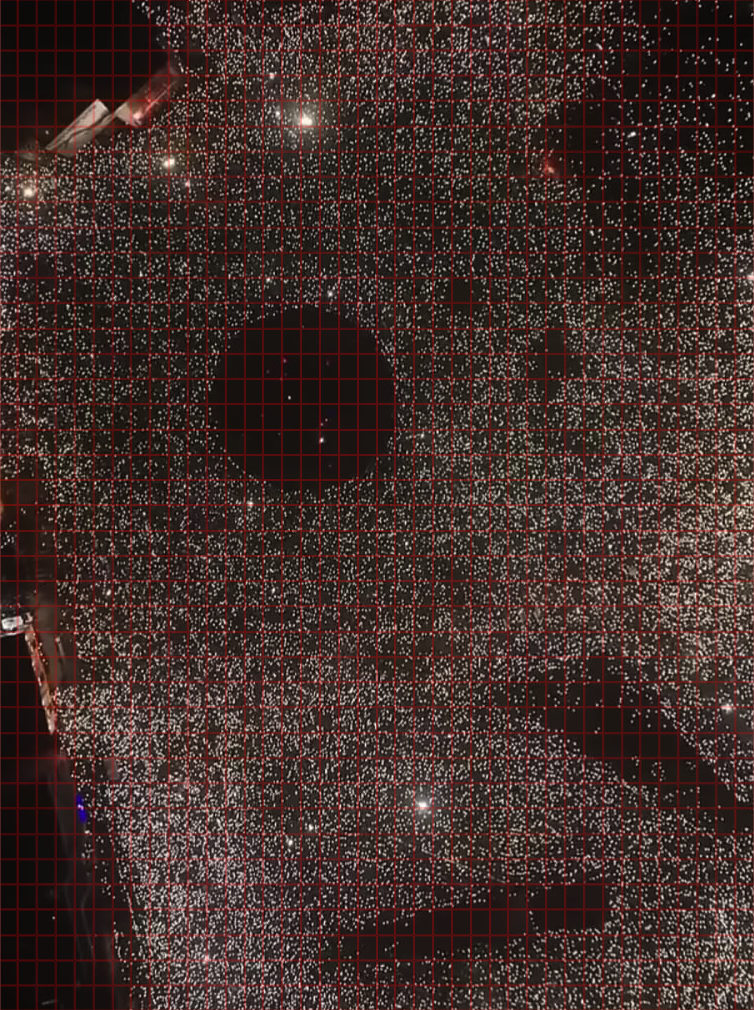
\includegraphics[width=0.8\textwidth]{../outputs/grid_output/slavija-centar_grid.png} 
	\caption{Slavija.} 
	\label{fig:slavija} 
\end{figure}

\begin{figure}[H]
	\centering
  
	% Prvi red
	\begin{subfigure}[b]{0.3\textwidth}
	  \centering
	  
\includegraphics[width=\textwidth]{../outputs/grid_output/prote-mateje_grid.png}
	  \caption{Prote Mateje}
	  \label{fig:prote-mateje}
	\end{subfigure}
	\hfill
	\begin{subfigure}[b]{0.3\textwidth}
	  \centering
	  
\includegraphics[width=\textwidth]{../outputs/grid_output/nemanjina_grid.png}
	  \caption{Nemanjina}
	  \label{fig:nemanjina}
	\end{subfigure}
	\hfill
	\begin{subfigure}[b]{0.3\textwidth}
		\centering
		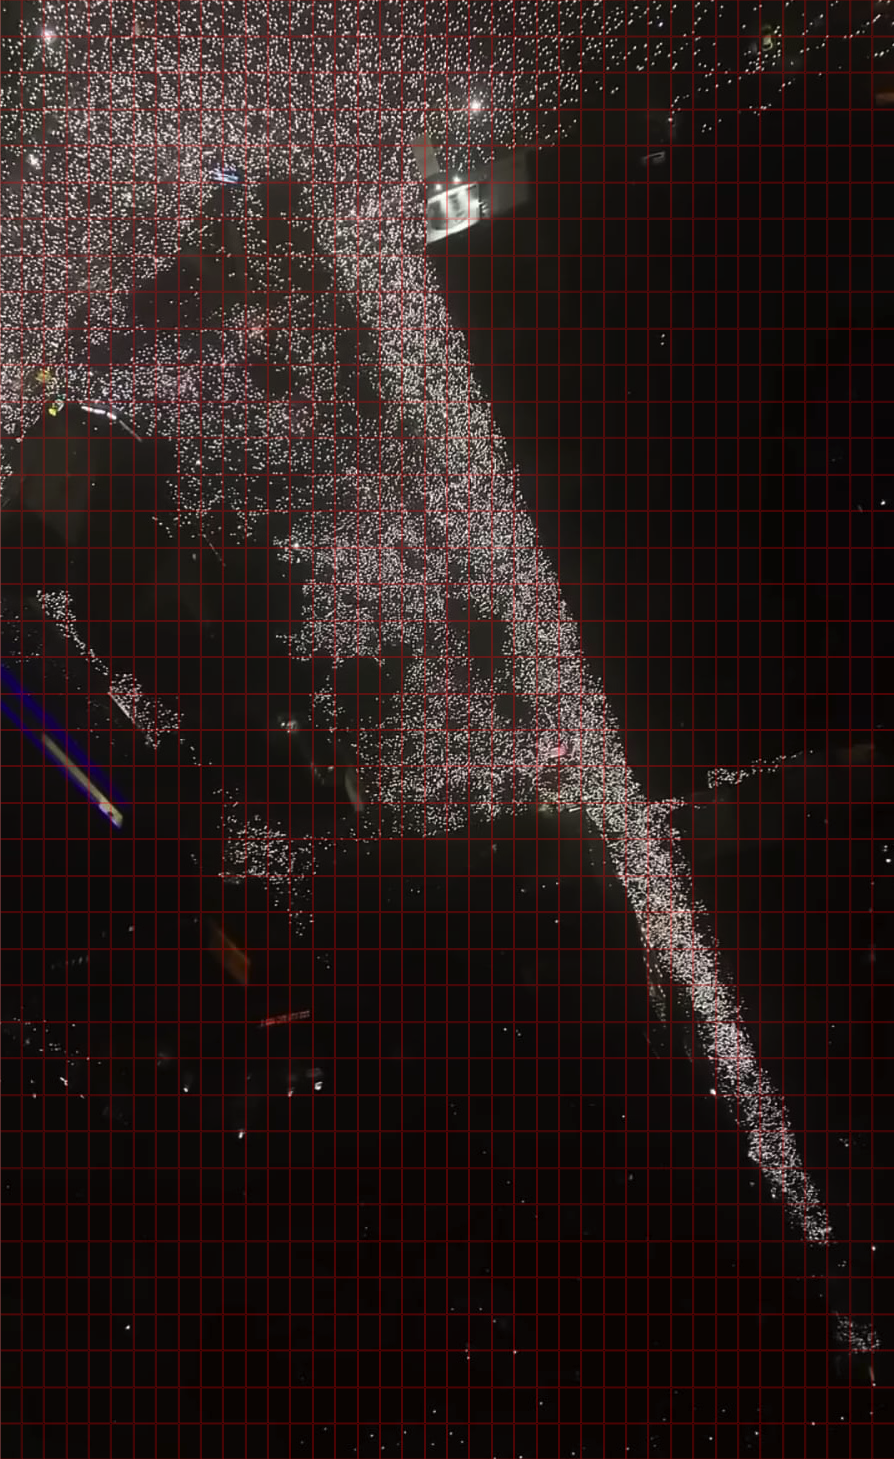
\includegraphics[width=\textwidth]{../outputs/grid_output/beogradska_grid.png}
		\caption{Beogradska}
		\label{fig:beogradska}
	\end{subfigure}
  
	\vspace{0.3cm} % razmak između redova
  
	% Drugi red
	\begin{subfigure}[b]{0.3\textwidth}
	  \centering
	  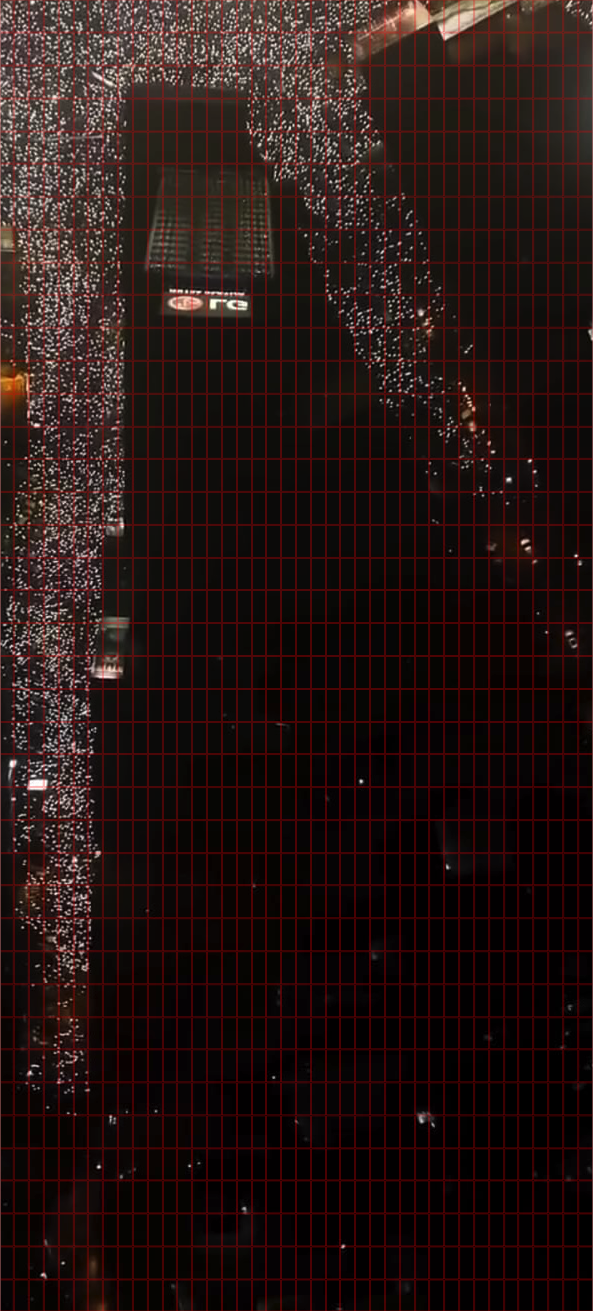
\includegraphics[width=\textwidth]{../outputs/grid_output/makenzijeva_grid.png}
	  \caption{Makenzijeva}
	  \label{fig:makenzijeva}
	\end{subfigure}
	\hfill
	\begin{subfigure}[b]{0.3\textwidth}
	  \centering
	  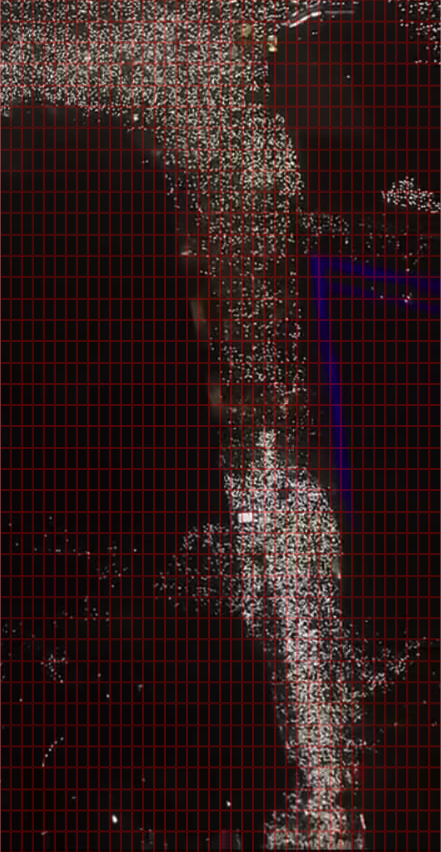
\includegraphics[width=\textwidth]{../outputs/grid_output/kralja-milana_grid.png}
	  \caption{Kralja Milana}
	  \label{fig:kralja-milana}
	\end{subfigure}
	\hfill
	\begin{subfigure}[b]{0.3\textwidth}
	  \centering
	  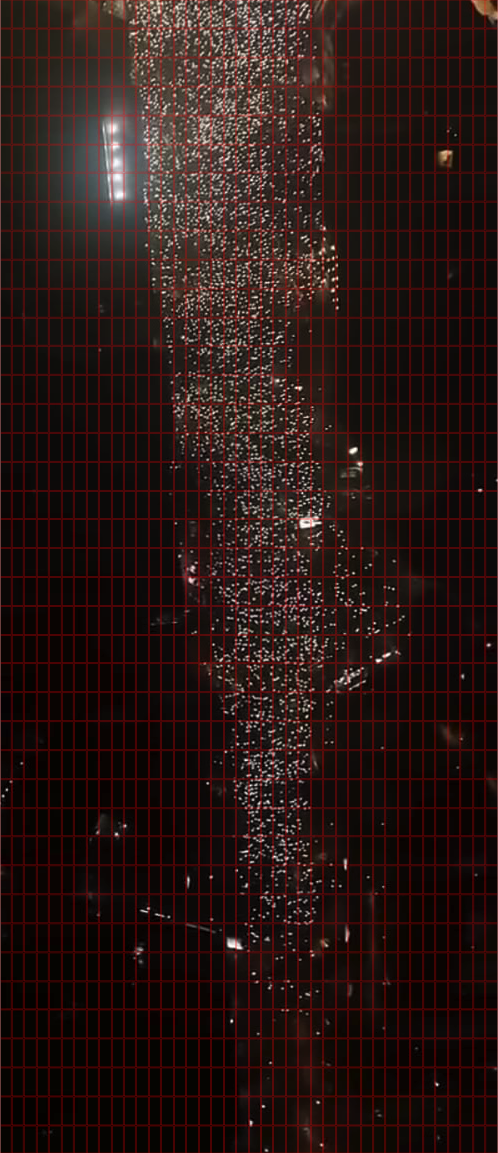
\includegraphics[width=\textwidth]{../outputs/grid_output/bulevar-oslobodjenja_grid.png}
	  \caption{Bulevar oslobođenja}
	  \label{fig:bulevar-oslobodjenja}
	\end{subfigure}
  
	\caption{Pregled ulica sa postavljenim grid-om}
\end{figure}

Radi smanjenja varijanse i troškova, uvodi se stratifikacija – grupisanje ćelija u tri stratuma (1 = najgušće, 2 = srednje, 3 = najređe).
Dodatno, gotovo „crne“ ćelije (bez informativnog sadržaja) sistematski se isključuju iz uzorkovanja.
\noindent
Dobijeni fajl \texttt{strata\_map\_auto.csv}, sa konačnim oznakama \texttt{include} i \texttt{stratum}, predstavlja osnovu za naredne korake – izbor pilot uzorka, primenu Neyman-ove alokacije i glavno uzorkovanje opisano u sledećim poglavljima, kao i za završnu procenu ukupnog broja ljudi.


\subsection{Automatska dodela stratuma (Python)}

Cilj je da automatski razvrstamo grid ćelije u 3 stratuma po gustini i pouzdano isključimo neinformativne oblasti radi manjeg troška uzorkovanja i niže varijanse ocene.
Skripta \texttt{stratum.py} za svaku ćeliju računa kompozitni skor gustine, koji kombinuje:
\begin{itemize}
    \item udeo svetlih piksela (\texttt{bright\_frac}),
    \item gustinu ivica (Canny edge detection),
    \item teksturnu varijansu (Laplacian variance).
\end{itemize}


\noindent Ulaz: \texttt{strata\_map.csv} (iz R grida) sa kolonama
\texttt{cell\_id, zone\_id, include, stratum, x0, x1, y0, y1, img\_path}.

\noindent Izlaz: \texttt{strata\_map\_auto.csv} — isto +
\texttt{strata\_score} (kompozitni skor), \texttt{black\_frac} (udeo “crnih” piksela), finalni include i stratum (1/2/3).
\newline
\newline
\noindent Ćelije kod kojih $ \ge 90\% $ piksela ima nisku osvetljenost (HSV V < 0.10) automatski se označavaju include = 0 i izuzimaju iz uzorkovanja. 
Preostale ćelije dele se na tri tercila po vrednosti kompozitnog skora: gornji tercil čini stratum 1, srednji stratum 2, a donji stratum 3.

\noindent
Automatska dodela se sastoji od sledećih koraka:
\begin{enumerate}
  \item \textbf{Maskiranje neinformativnih ćelija:} svaka ćelija se ispituje u HSV prostoru boja. Ako je udeo piksela sa niskom vrednošću osvetljenja (V) veći od zadatog praga (\texttt{black\_frac}, npr.\ 90\%), ćelija se automatski označava kao \texttt{include = 0}.
  \item \textbf{Računanje metrika:} za sve preostale ćelije izračunavaju se tri nezavisne metrike – udeo svetlih piksela (\texttt{bright\_frac}), gustina ivica (Canny edge detection) i teksturna varijansa (Laplacian variance).
  \item \textbf{Kombinovanje u kompozitni skor:} konačan \texttt{strata\_score} dobija se linearnom kombinacijom metrika sa težinama 0.4, 0.4 i 0.2.
  \item \textbf{Dodela stratuma:} ćelije sa \texttt{include = 1} dele se na tercile prema \texttt{strata\_score} (1 = gornji tercil, 2 = srednji, 3 = donji).
\end{enumerate}

\noindent
Najvažniji parametri skripte su prag za crnu boju \texttt{v\_black}, udeo crnih piksela \texttt{black\_frac}, prag za svetle piksele \texttt{v\_thresh}, prag zasićenja \texttt{s\_thresh}, kao i kvantil \texttt{low\_score\_q} za dodatno isključivanje najslabijih ćelija.

\subsection{Vizuelna provera stratuma (R)}

Rezultati automatske dodele vizuelizuju se, koja za svaku sliku prikazuje grid sa ćelijama obojenim po stratumu i zasenčenim poljima koja su isključena (include=0).
Crveno obojene su ćelije najveće gustine - stratum = 1, žute su ćelije srednje gustine - stratum = 2, zelene ćelije najmanje gustine - stratum = 3.
\newline
\noindent
Ovaj vizuelni korak služi kao brza kontrola kvaliteta: ukoliko se uoči da je algoritam označio kao gušće delove koji su u stvarnosti prazni (ili obrnuto), moguće je ručno prilagoditi vrednosti parametara i ponoviti automatsku dodelu.

\begin{figure}[H] 
	\centering 
	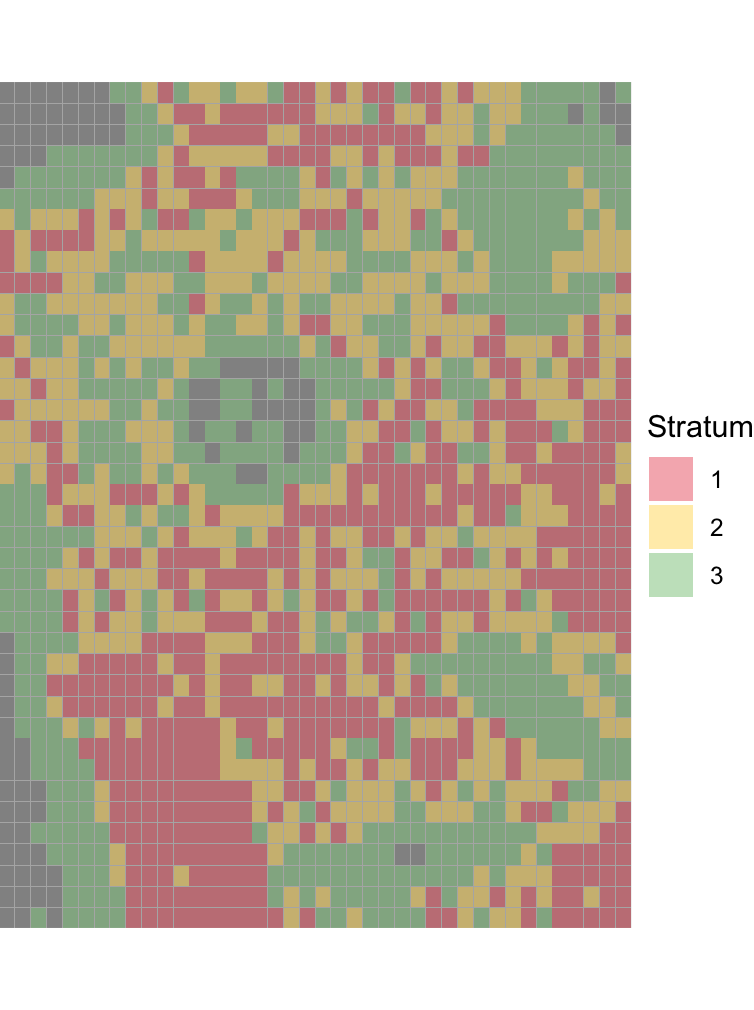
\includegraphics[width=0.8\textwidth]{../outputs/grid_output/strata_viz/slavija-centar_strata.png} 
	\caption{Slavija.} 
	\label{fig:slavija} 
\end{figure}

\begin{figure}[H]
	\centering
  
	% Prvi red
	\begin{subfigure}[b]{0.3\textwidth}
	  \centering
	  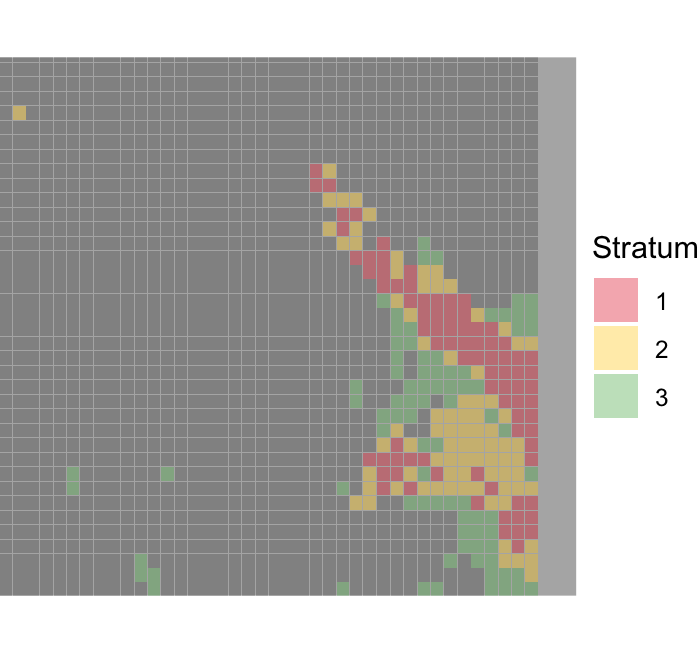
\includegraphics[width=\textwidth]{../outputs/grid_output/strata_viz/prote-mateje_strata.png}
	  \caption{Prote Mateje}
	  \label{fig:prote-mateje}
	\end{subfigure}
	\hfill
	\begin{subfigure}[b]{0.3\textwidth}
	  \centering
	  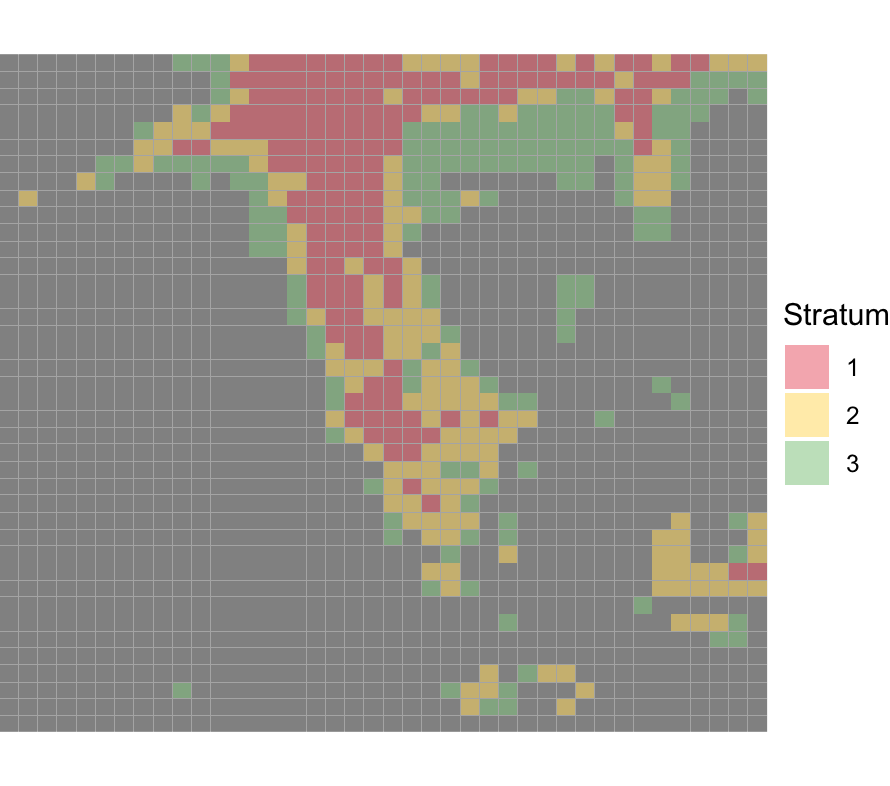
\includegraphics[width=\textwidth]{../outputs/grid_output/strata_viz/nemanjina_strata.png}
	  \caption{Nemanjina}
	  \label{fig:nemanjina}
	\end{subfigure}
	\hfill
	\begin{subfigure}[b]{0.3\textwidth}
		\centering
		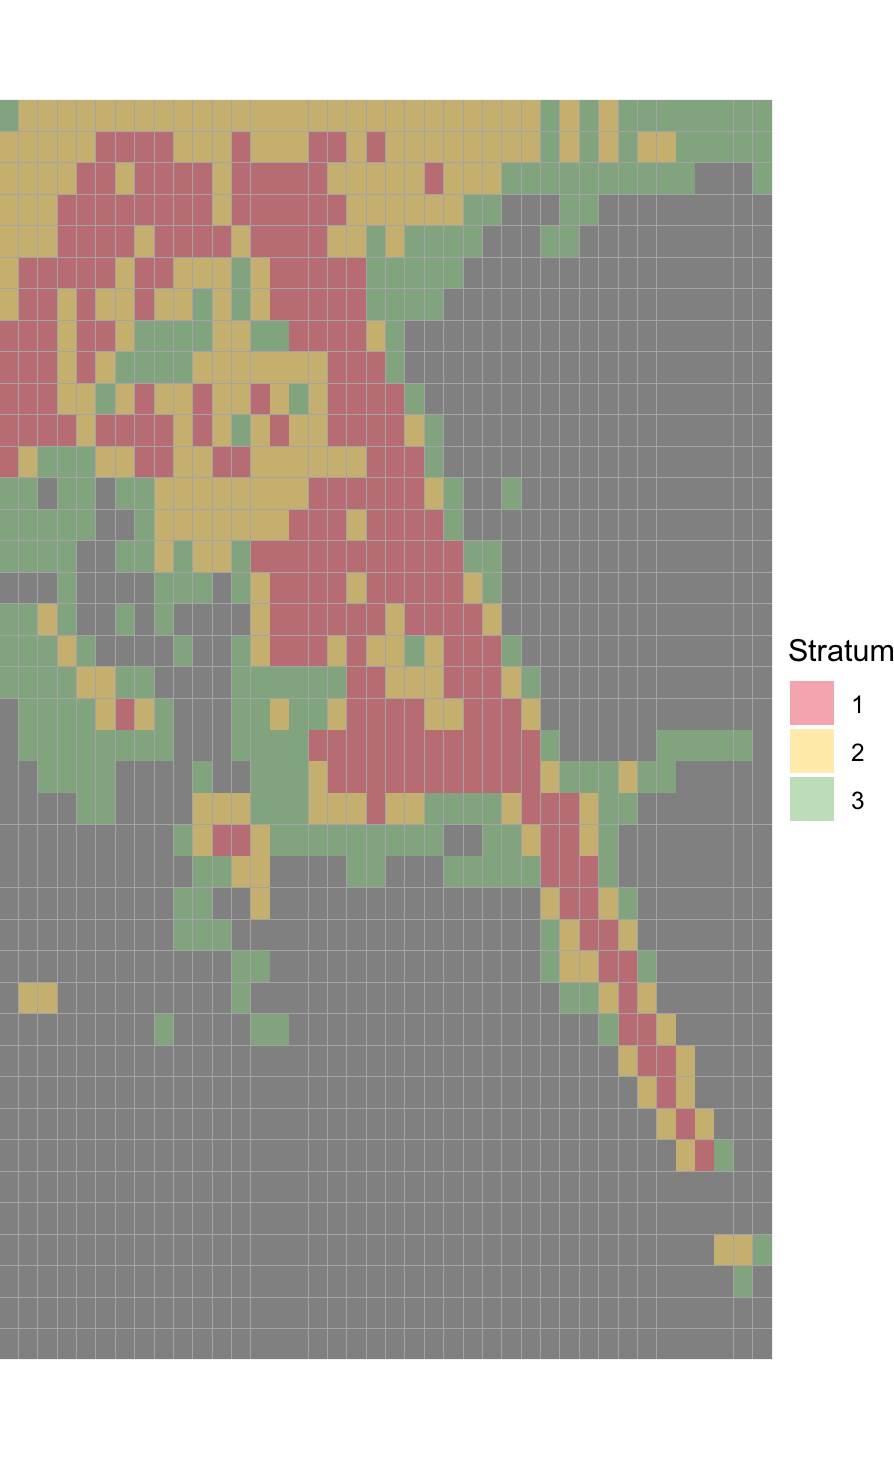
\includegraphics[width=\textwidth]{../outputs/grid_output/strata_viz/beogradska_strata.png}
		\caption{Beogradska}
		\label{fig:beogradska}
	\end{subfigure}
  
	\vspace{0.3cm} % razmak između redova
  
	% Drugi red
	\begin{subfigure}[b]{0.3\textwidth}
	  \centering
	  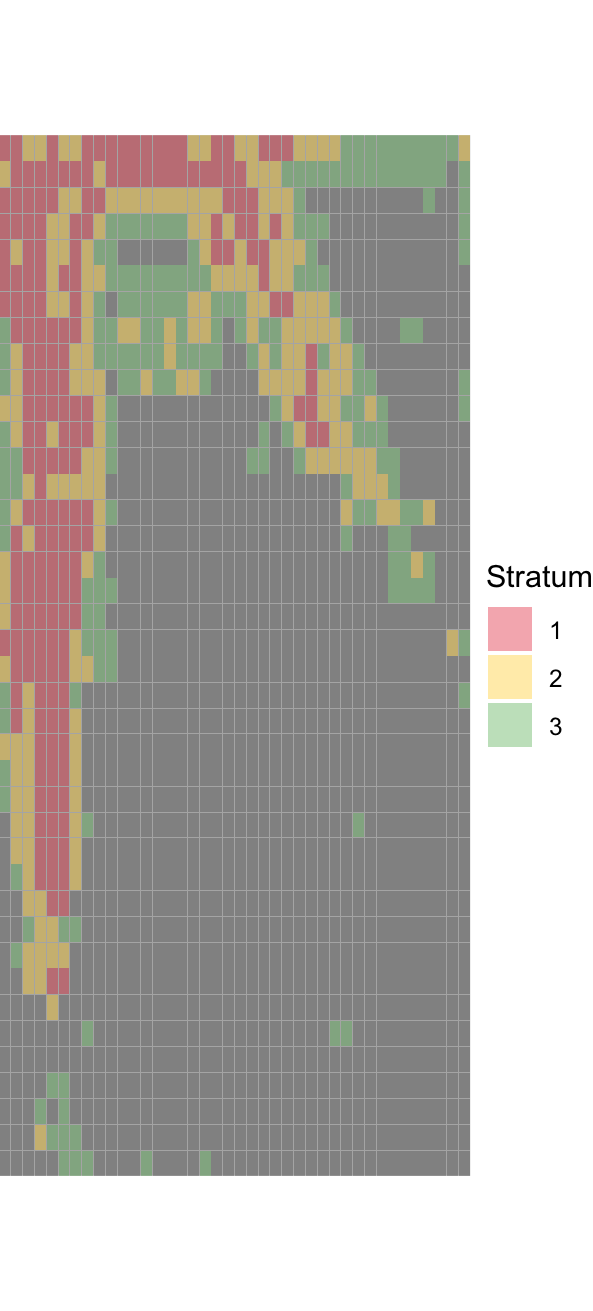
\includegraphics[width=\textwidth]{../outputs/grid_output/strata_viz/makenzijeva_strata.png}
	  \caption{Makenzijeva}
	  \label{fig:makenzijeva}
	\end{subfigure}
	\hfill
	\begin{subfigure}[b]{0.3\textwidth}
	  \centering
	  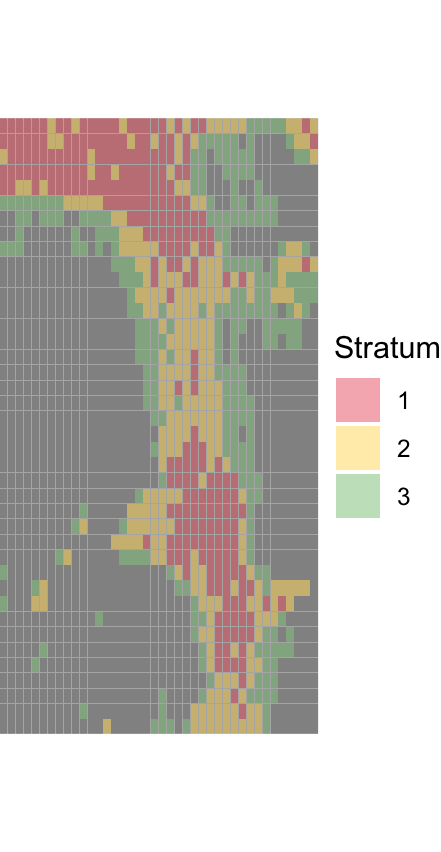
\includegraphics[width=\textwidth]{../outputs/grid_output/strata_viz/kralja-milana_strata.png}
	  \caption{Kralja Milana}
	  \label{fig:kralja-milana}
	\end{subfigure}
	\hfill
	\begin{subfigure}[b]{0.3\textwidth}
	  \centering
	  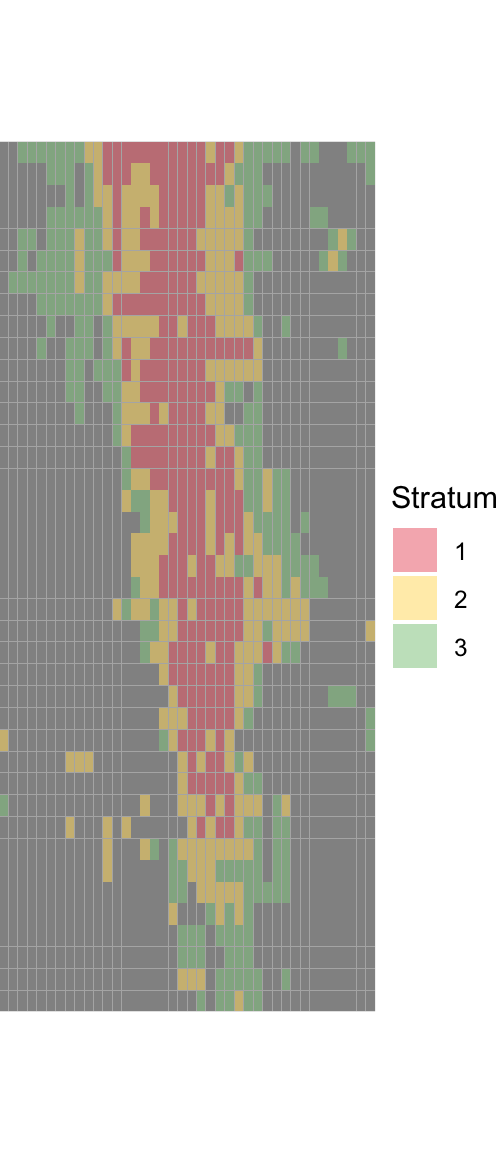
\includegraphics[width=\textwidth]{../outputs/grid_output/strata_viz/bulevar-oslobodjenja_strata.png}
	  \caption{Bulevar oslobođenja}
	  \label{fig:bulevar-oslobodjenja}
	\end{subfigure}
  
	\caption{Pregled ćelija po stratumima različitih gustina}
\end{figure}

\noindent
Nakon vizuelne provere i eventualnih korekcija, \texttt{strata\_map\_auto.csv} se koristi kao pouzdana ulazna baza za statističku analizu i uzorkovanje.

\section{Pilot uzorak i Neyman}

\subsection{Pilot uzorak}

U okviru implementacije uzorkovanja (\texttt{sampling\_pipeline.R} datoteka), 
prvi korak je izdvajanje pilot uzorka iz svakog stratuma. 
Za svaku sliku, unutar svakog sloja nasumično se bira fiksan broj jedinica 
(\texttt{pilot\_n\_per\_stratum}), koji u ovom primeru iznosi $15$. Broj odabranih jedinica u pilot fazi ($n_h = 15$ u ovom primeru) predstavlja kompromis između 
dovoljno velike veličine za pouzdane procene i ograničavanja troška uzorkovanja.
Na ovaj način dobija se preliminarni uzorak dovoljan da se procene osnovne 
karakteristike slojeva, poput srednje vrednosti i disperzije.

Procene iz pilot uzorka koriste se da bi se izračunale disperzije unutar slojeva. 
Za sloj $h$ disperzija se računa po formuli:
\[
s_h^2 = \frac{1}{n_h - 1} \sum_{i=1}^{n_h} (y_i - \bar{y}_h)^2,
\]
gde je $\bar{y}_h$ srednja vrednost pilot uzorka u sloju $h$, a $n_h$ veličina pilot uzorka u tom sloju.

Dobijene procene standardne devijacije $\hat{S}_h = \sqrt{s_h^2}$ 
koriste se u narednom koraku, prilikom određivanja optimalne raspodele ukupnog 
uzorka po slojevima primenom Neymanove alokacije.
\subsubsection{Vizuelizacija pilot uzorka}

Uz CSV \texttt{pilot\_to\_count.csv}, za svaku ulaznu sliku generišemo i PNG sa označenim ćelijama pilota. Na overlay-ima:
\begin{itemize}
	\item cela slika je prikazana,
	\item zelenim okvirima su označene ćelije koje su ušle u pilot uzorak.
\end{itemize}

\begin{figure}[H] 
	\centering 
	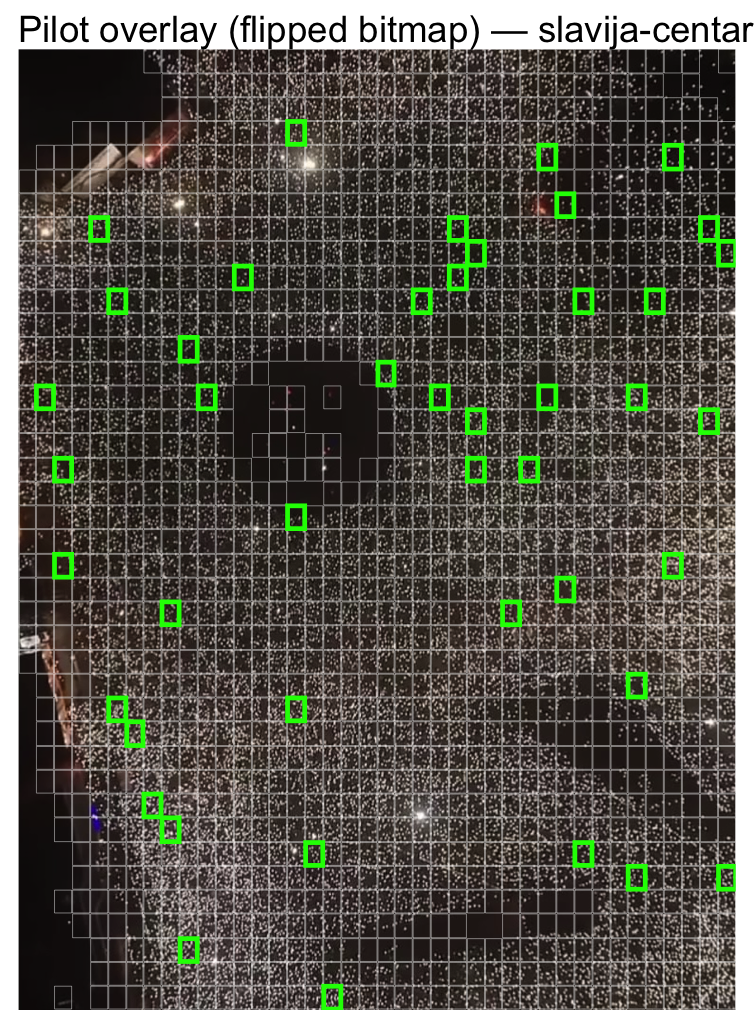
\includegraphics[width=0.8\textwidth]{../outputs/sampling_outputs/plot_overlays_image/pilot_overlay_slavija-centar.png} 
	\caption{Slavija.} 
	\label{fig:slavija} 
\end{figure}

\begin{figure}[H]
	\centering
  
	% Prvi red
	\begin{subfigure}[b]{0.3\textwidth}
	  \centering
	  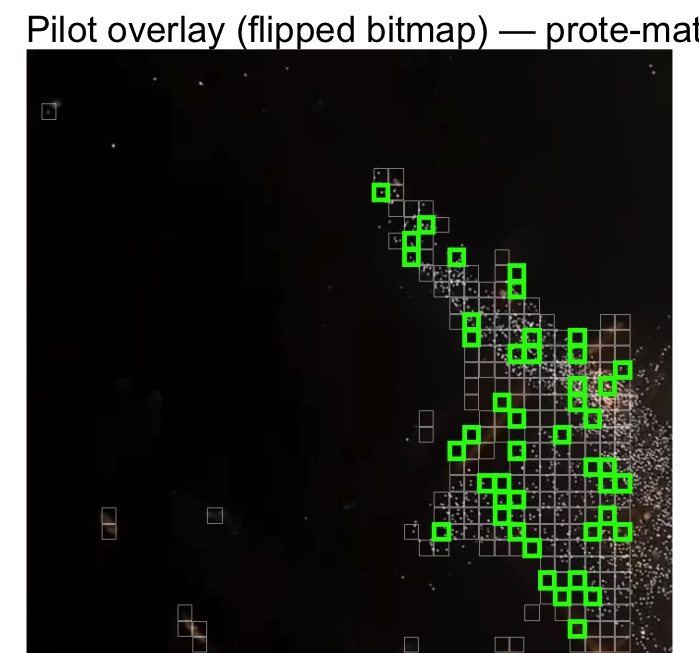
\includegraphics[width=\textwidth]{../outputs/sampling_outputs/plot_overlays_image/pilot_overlay_prote-mateje.png}
	  \caption{Prote Mateje}
	  \label{fig:prote-mateje}
	\end{subfigure}
	\hfill
	\begin{subfigure}[b]{0.3\textwidth}
	  \centering
	  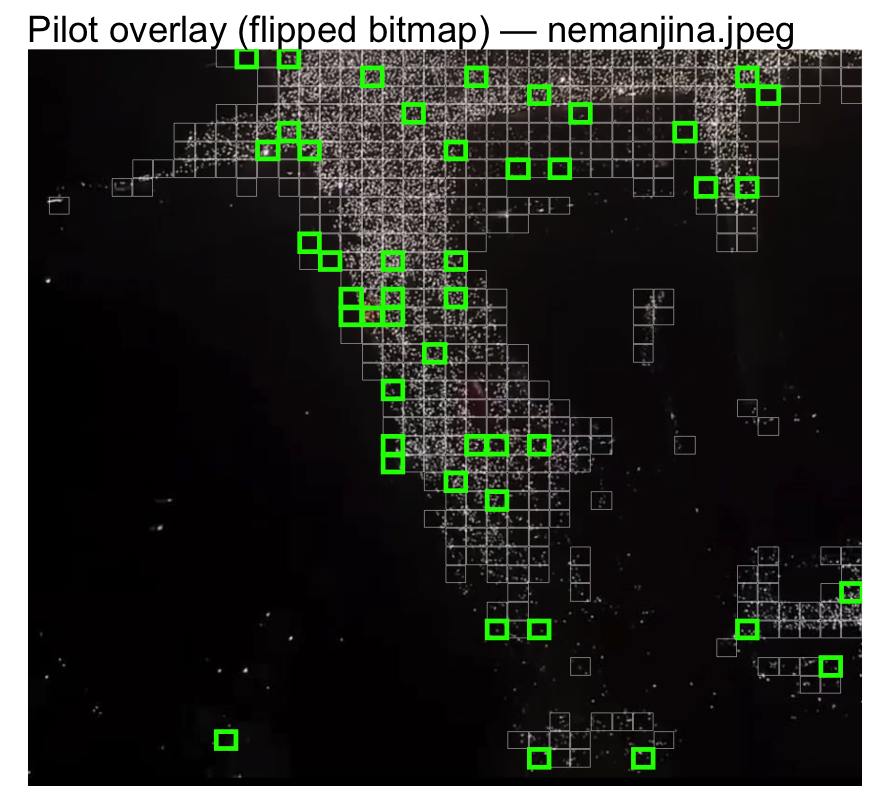
\includegraphics[width=\textwidth]{../outputs/sampling_outputs/plot_overlays_image/pilot_overlay_nemanjina.png}
	  \caption{Nemanjina}
	  \label{fig:nemanjina}
	\end{subfigure}
	\hfill
	\begin{subfigure}[b]{0.3\textwidth}
		\centering
		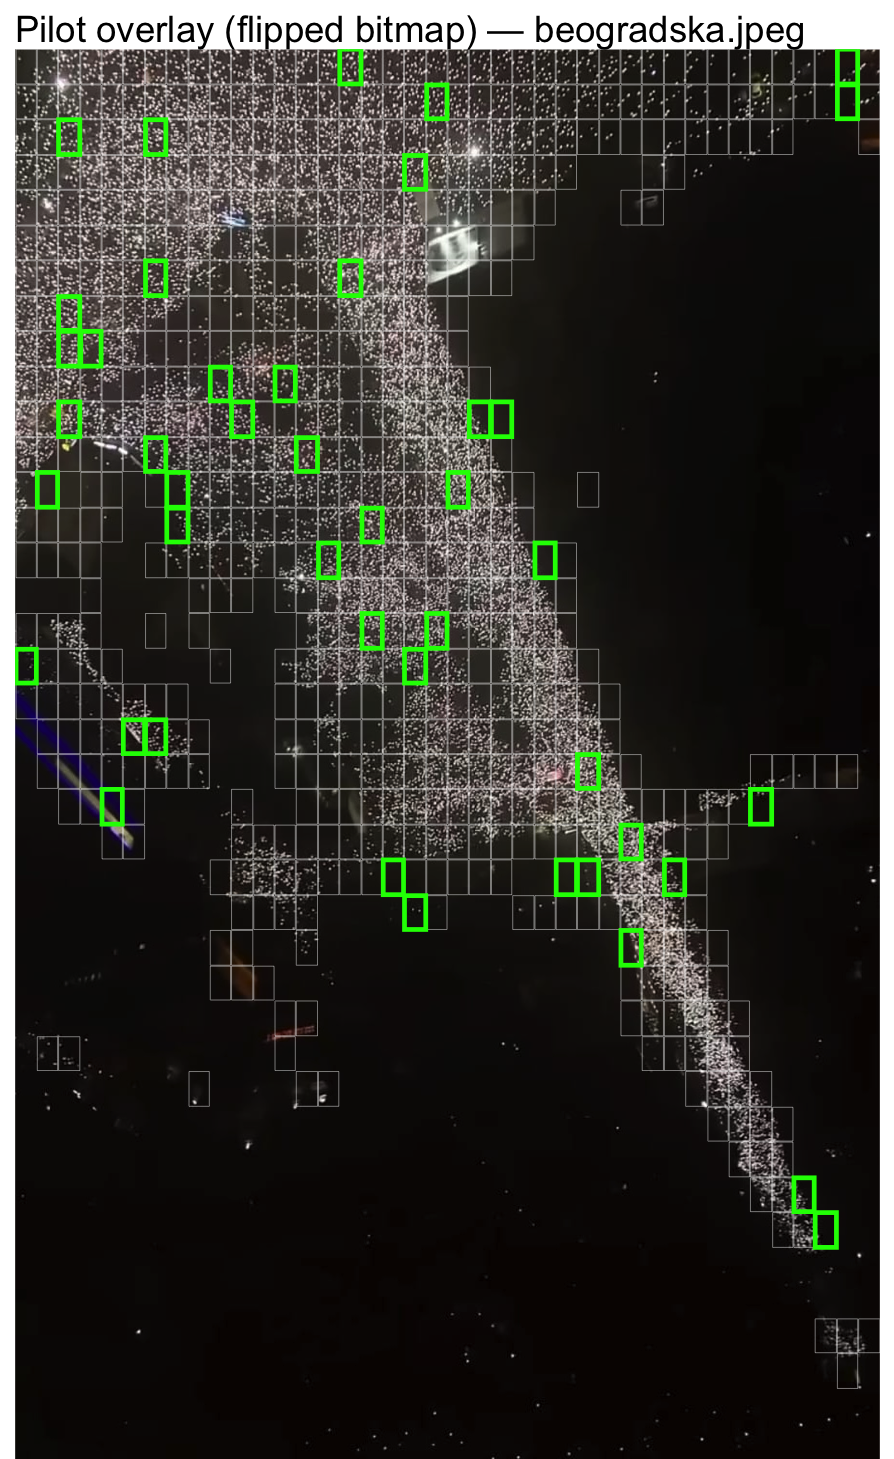
\includegraphics[width=\textwidth]{../outputs/sampling_outputs/plot_overlays_image/pilot_overlay_beogradska.png}
		\caption{Beogradska}
		\label{fig:beogradska}
	\end{subfigure}
  
	\vspace{0.3cm} % razmak između redova
  
	% Drugi red
	\begin{subfigure}[b]{0.3\textwidth}
	  \centering
	  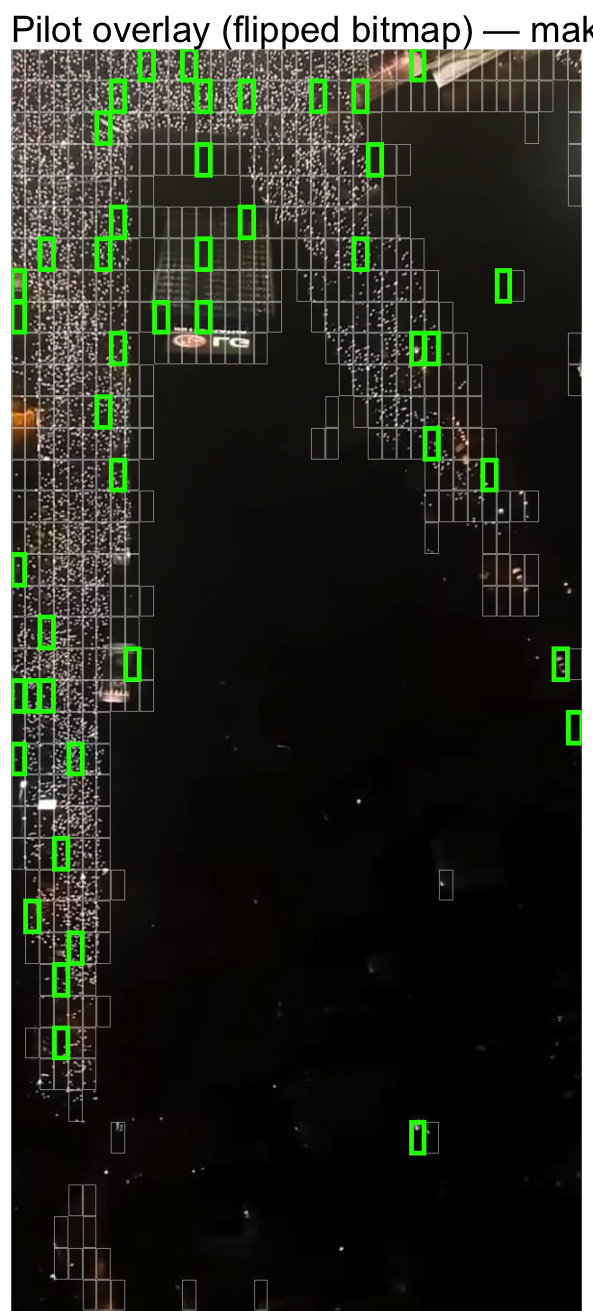
\includegraphics[width=\textwidth]{../outputs/sampling_outputs/plot_overlays_image/pilot_overlay_makenzijeva.png}
	  \caption{Makenzijeva}
	  \label{fig:makenzijeva}
	\end{subfigure}
	\hfill
	\begin{subfigure}[b]{0.3\textwidth}
	  \centering
	  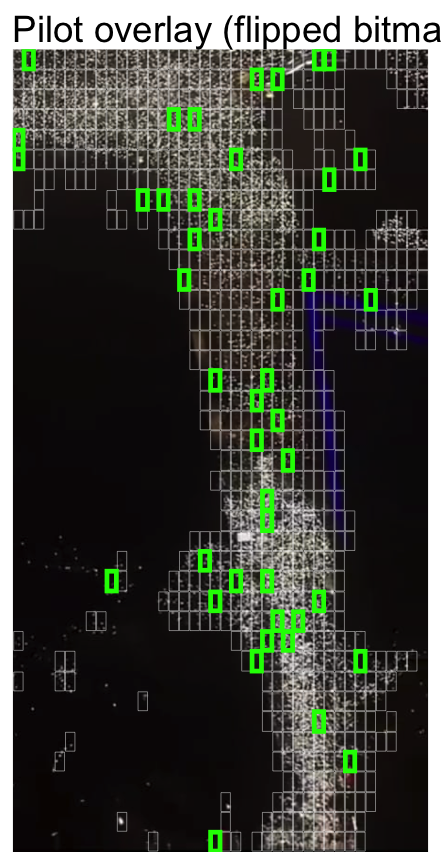
\includegraphics[width=\textwidth]{../outputs/sampling_outputs/plot_overlays_image/pilot_overlay_kralja-milana.png}
	  \caption{Kralja Milana}
	  \label{fig:kralja-milana}
	\end{subfigure}
	\hfill
	\begin{subfigure}[b]{0.3\textwidth}
	  \centering
	  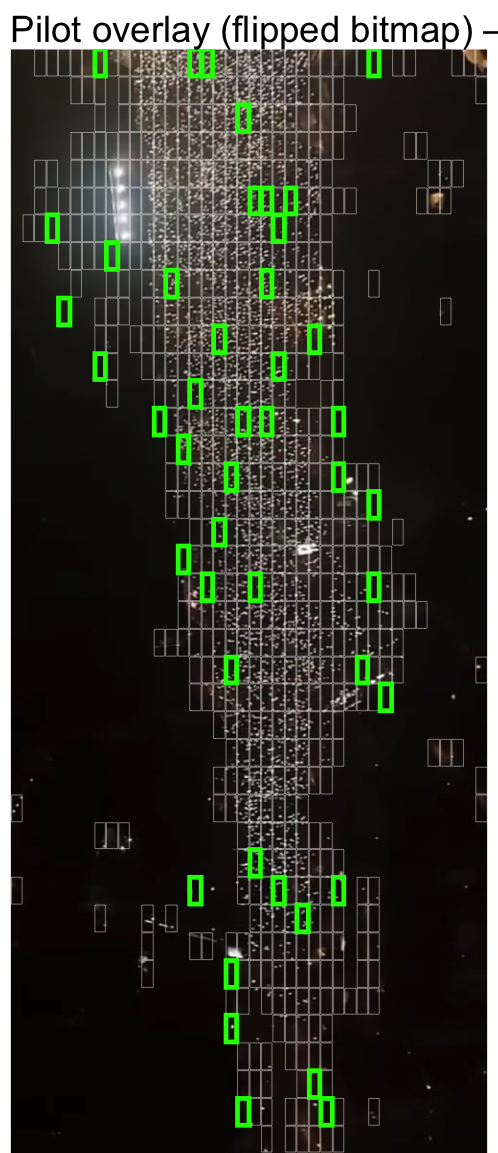
\includegraphics[width=\textwidth]{../outputs/sampling_outputs/plot_overlays_image/pilot_overlay_bulevar-oslobodjenja.png}
	  \caption{Bulevar oslobođenja}
	  \label{fig:bulevar-oslobodjenja}
	\end{subfigure}
  
	\caption{Prikaz preklopa (overlay) pilot ćelija preko svake slike}
\end{figure}

\noindent
Ovaj vizuelni prikaz će nam omogućiti da lakše odredimo u kojim ćelijama brojimo bliceve. 
Kako bismo popunili napravljeni CSV, koristićemo automatsko brojanje bliceva pomoću python skripte \texttt{auto-count.py}, o kojoj će biti više
reči u narednom poglavlju. Dodatno za neke ćelije koristili smo ručno brojanje.

\subsection{Neymanov metod raspodele obima uzorka po stratumima}
\noindent

Cilj Neymanove alokacije je da za fiksni ukupan broj uzoraka $n$ raspodeli broj uzorkovanih jedinica $n_h$ po stratumima tako da se minimizuje varijansa procene ciljnog parametra.  
Za jednu sliku, disperzija procene totalne sume $\hat T$ glasi
\[
\mathrm{Var}(\hat T) \;=\; \sum_{h=1}^H N_h^2 \left(1-\frac{n_h}{N_h}\right)\frac{S_h^2}{n_h},
\]
gde je $N_h$ veličina populacije (broj ćelija) u stratumu $h$, $n_h$ broj izabranih ćelija u tom stratumu, a $S_h^2$ varijansa u stratumu $h$ (procena se dobija iz pilot uzorka).  

U praksi se često radi aproksimacija koja zanemaruje faktor konačne populacije $(1 - n_h/N_h)$ (što je opravdano kada su frakcije uzorkovanja male), pa se kao cilj minimizuje
\[
\sum_{h=1}^H \frac{N_h^2 S_h^2}{n_h}.
\]
Pošto mora važiti uslov
\[
\sum_{h=1}^H n_h = n,
\]
Kako bismo rešili problem sa ograničenjem, uvodimo Lagranžov množilac $\lambda$ i formiramo funkciju
\[
L(n_1, \dots, n_H, \lambda) = \sum_{h=1}^H \frac{N_h^2 S_h^2}{n_h} 
+ \lambda \left( \sum_{h=1}^H n_h - n \right).
\]
Računamo parcijalni izvod po $n_h$:
\[
\frac{\partial L}{\partial n_h} = -\frac{N_h^2 S_h^2}{n_h^2} + \lambda = 0.
\]

Iz ovog dobijamo
\[
\frac{N_h^2 S_h^2}{n_h^2} = \lambda
\quad \Rightarrow \quad
n_h = \frac{N_h S_h}{\sqrt{\lambda}}.
\]

Obim uzorka po stratumu je proporcionalan proizvodu $N_h S_h$.


Dakle, klasična Neymanova alokacija glasi
\[
\boxed{ \; n_h \;=\; n \cdot \frac{N_h S_h}{\sum_{j=1}^H N_j S_j} \; }.
\]

\paragraph{Intuicija.} Stratumu $h$ dodeljuje se više jedinica ako je ili veliki ($N_h$ veliko) ili veoma varijabilan ($S_h$ veliko). Time se uzorci usmeravaju tamo gde će imati najveći doprinos smanjenju ukupne varijanse procene.

\paragraph{Praktične napomene pri implementaciji}
\begin{itemize}
  \item \textbf{Procena $S_h$.} Standardne devijacije $S_h$ su obično nepoznate pre pilot uzorka — zato se u praksi koriste procene $\hat S_h$ iz pilot faze.
  \item \textbf{Zaokruživanje i diskretizacija.} Formula daje realne brojeve; potrebno je zaokružiti na celi broj. Zaokruživanje može uvesti residual (suma $n_h$ možda nije tačno $n$).
  \item \textbf{Ograničenja:} ne smemo dodeliti više jedinica nego što postoji ($n_h \le N_h$), niti manje od minimalnog prihvatljivog broja ($n_h \ge n_{\min}$) ako smo takav prag uveli.
  \item \textbf{Posebni slučajevi:} ako su sve procene varijanse jednake nuli (npr.\ nema detekcija u pilotu), koristi se alternativna alokacija npr.\ proporcionalna $N_h$.
  \item \textbf{Popravka (balansiranje):} zbog zaokruživanja suma $\sum_h n_h$ može odstupati od $n$. U radu primenjujemo jednostavnu korekciju.
\end{itemize}

\paragraph{Algoritamski koraci (kako je izvedeno u kodu)}
\begin{enumerate}
  \item Iz pilot uzorka izračunati $\hat S_h$ za svaki stratuma i dobiti $N_h$ (broj ćelija u stratumu, po slici).
  \item Za svaku sliku izračunati težine $w_h = N_h \hat S_h$ i formirati početnu alokaciju
  \[
  n_h^{(0)} = \mathrm{round}\!\Big( n \cdot \frac{w_h}{\sum_j w_j} \Big).
  \]
  Ako $\sum_j w_j = 0$, alokacija se radi proporcionalno $N_h$.
  \item Primeniti ograničenja: $n_h \leftarrow \min\{ \max(n_h, n_{\min}), N_h\}$.
  \item Izračunati \texttt{diff} = $n - \sum_h n_h$. Primeniti malu korekciju.
\end{enumerate}

\paragraph{Isečak R-koda} (preuzet iz sampling\_pipeline.R)
\begin{verbatim}
# Neyman allocation vector for one image
neyman_alloc_vec <- function(Nh, sh, n_total, n_min=10) {
  Nh <- as.numeric(Nh); sh <- as.numeric(sh)
  w <- Nh * sh
  if (sum(w) > 0) nh <- round(n_total * w / sum(w)) 
  else nh <- round(n_total * Nh / sum(Nh))
  nh <- pmax(nh, pmin(n_min, Nh))
  nh <- pmin(nh, Nh)
  nh
}
\end{verbatim}

Zbog zaokruživanja često se dešava da zbir po stratumima odstupa od ciljne veličine uzorka $n$:
\[
\sum_h n_h \;\neq\; n.
\]
Taj višak ili manjak može biti nekoliko jedinica, a ne sme se ignorisati jer remeti planirano uzorkovanje.
Zato uvodimo malu popravku (balansiranje) kako bismo tačno pogodili cilj:
\begin{itemize}
  \item Izračunava se razlika od cilja:
  \[
  \text{diff} = n - \sum_h n_h.
  \]
  \item Popravka se primenjuje u \textbf{stratumu 1} (najgušći), jer taj stratum obično najviše doprinosi varijansi. 
  \item Ako je $\text{diff} > 0$ (fali uzoraka) i $n_1 < N_1$, dodaje se $\min(\text{diff}, N_1 - n_1)$ u stratumu 1.
  \item Ako je $\text{diff} < 0$ (ima viška) i $n_1 > \min(n_{\min}, N_1)$, oduzima se $\min(-\text{diff}, n_1 - n_{\min})$.
\end{itemize}

\noindent
Nakon primene Neymanove alokacije, ukupni brojevi uzoraka po slici su prikazani u Tabeli \ref{tab:alloc-fix-real}.  
Vidimo da su kod većine slika ukupni brojevi tačno jednaki cilju $n=180$, dok su kod dve slike odstupali za $\pm 1$.  
U skladu sa procedurom popravke, razlika je uvek ispravljena unutar stratuma 1, tako da je konačan broj uzoraka po slici tačno $n=180$.

\begin{table}[H]
\centering
\begin{tabular}{lccc}
\hline
Slika & Total pre & Target & Total posle \\
\hline
beogradska.jpeg          & 179 & 180 & 180 \\
bulevar-oslobodjenja.jpeg & 179 & 180 & 180 \\
kralja-milana.jpeg       & 180 & 180 & 180 \\
makenzijeva.jpeg         & 180 & 180 & 180 \\
nemanjina.jpeg           & 180 & 180 & 180 \\
prote-mateje.jpeg        & 181 & 180 & 180 \\
slavija-centar.jpeg      & 180 & 180 & 180 \\
\hline
\end{tabular}
\caption{Ukupni brojevi uzoraka po slici pre i posle korekcije.}
\label{tab:alloc-fix-real}
\end{table}

\noindent
U Tabeli \ref{tab:alloc-beogradska} prikazana je raspodela uzorka po stratumima za sliku \texttt{beogradska.jpeg}.  
Vidimo da je zbir po stratumima iznosio $179$ (umesto ciljanih $180$).  
Korekcijom je dodata jedna jedinica u stratumu 1, tako da se ukupni broj uzoraka uskladio sa ciljem.

\begin{table}[H]
\centering
\begin{tabular}{lcccc}
\hline
Stratum & $n_h$ (pre) & $N_h$ & Diff & $n_h$ (posle) \\
\hline
1 & 55 & 226 & +1 & 56 \\
2 & 51 & 226 & 0  & 51 \\
3 & 73 & 226 & 0  & 73 \\
\hline
\textbf{Ukupno} & 179 & 678 & +1 & 180 \\
\hline
\end{tabular}
\caption{Primer raspodele po stratumima za sliku beogradska.jpeg (pre i posle korekcije).}
\label{tab:alloc-beogradska}
\end{table}

\section{Glavno uzorkovanje i brojanje “bliceva”}

Nakon završene pilot faze i određivanja optimalne raspodele jedinica po slojevima, 
sledi glavno uzorkovanje. Ideja glavnog uzorka jeste da se iz svakog sloja odabere 
onaj broj jedinica koji je unapred određen pomoću Neymanove alokacije. 
Na taj način obezbeđuje se da slojevi sa većom veličinom ($N_h$) i većom varijabilnošću ($s_h$) 
dobiju veći broj jedinica, dok slojevi sa manjom varijabilnošću ili obimom dobijaju manje. 
Ova strategija značajno povećava efikasnost procene u odnosu na proporcionalnu alokaciju, 
jer omogućava da se ograničeni broj jedinica iskoristi na onim mestima gde najviše doprinose 
smanjenju ukupne varijanse.

Dobijeni uzorak se na kraju čuva u datoteci 
\texttt{main\_to\_count.csv} i koristi za dalju analizu i procene.

\subsection{Vizuelizacija glavnog uzorkovanja}

Uz CSV \texttt{main\_to\_count.csv}, za svaku ulaznu sliku generišemo i PNG sa označenim ćelijama glavnog uzorka. Na overlay-ima:
\begin{itemize}
	\item cela slika je prikazana,
	\item zelenim okvirima su označene ćelije koje su ušle u glavni uzorak.
\end{itemize}

\begin{figure}[H] 
	\centering 
	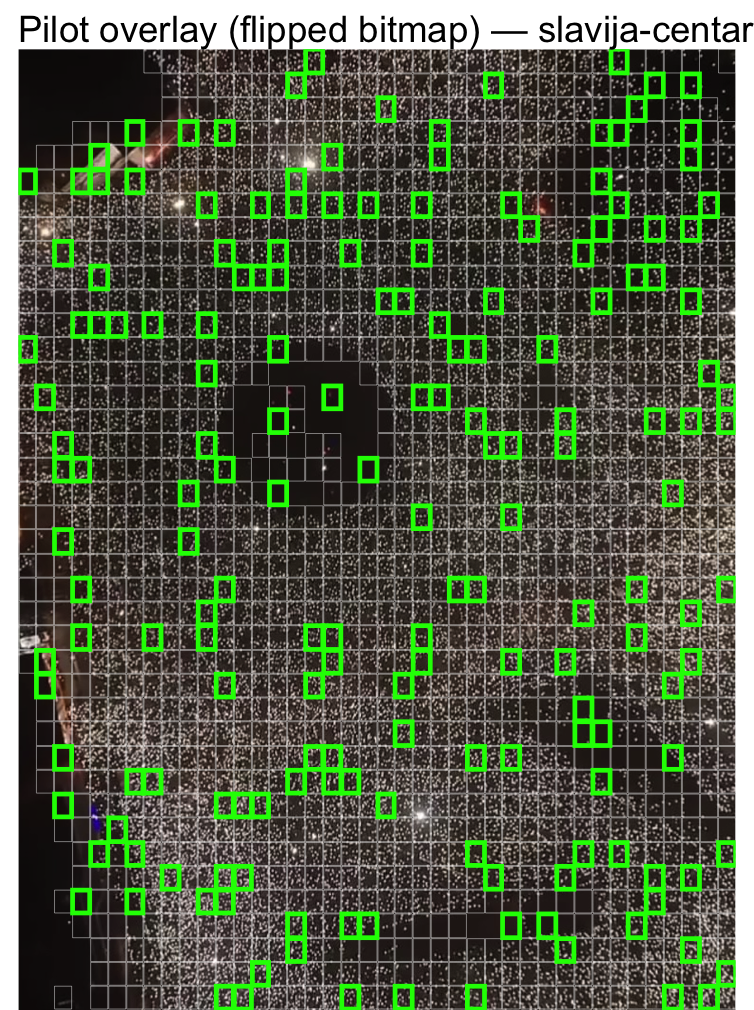
\includegraphics[width=0.8\textwidth]{../outputs/sampling_outputs/main_overlays_image/main_overlay_slavija-centar.png} 
	\caption{Slavija.} 
	\label{fig:slavija} 
\end{figure}

\begin{figure}[H]
	\centering
  
	% Prvi red
	\begin{subfigure}[b]{0.3\textwidth}
	  \centering
	  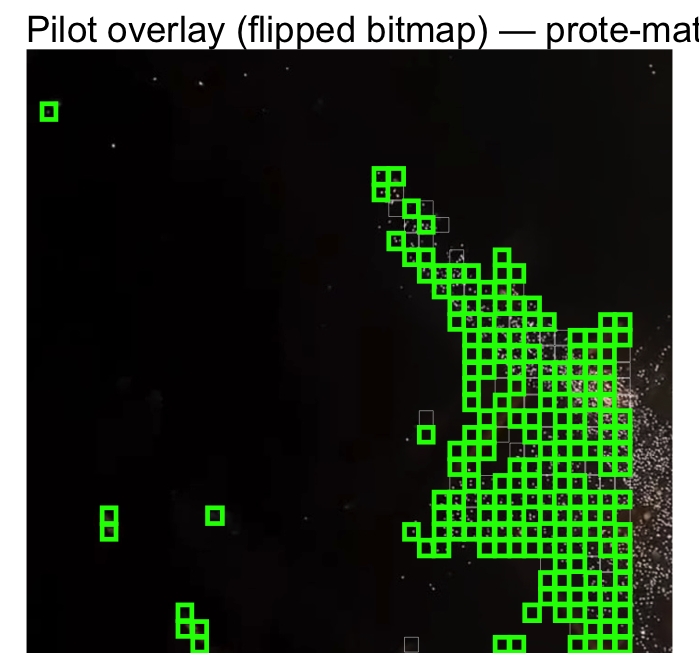
\includegraphics[width=\textwidth]{../outputs/sampling_outputs/main_overlays_image/main_overlay_prote-mateje.png}
	  \caption{Prote Mateje}
	  \label{fig:prote-mateje}
	\end{subfigure}
	\hfill
	\begin{subfigure}[b]{0.3\textwidth}
	  \centering
	  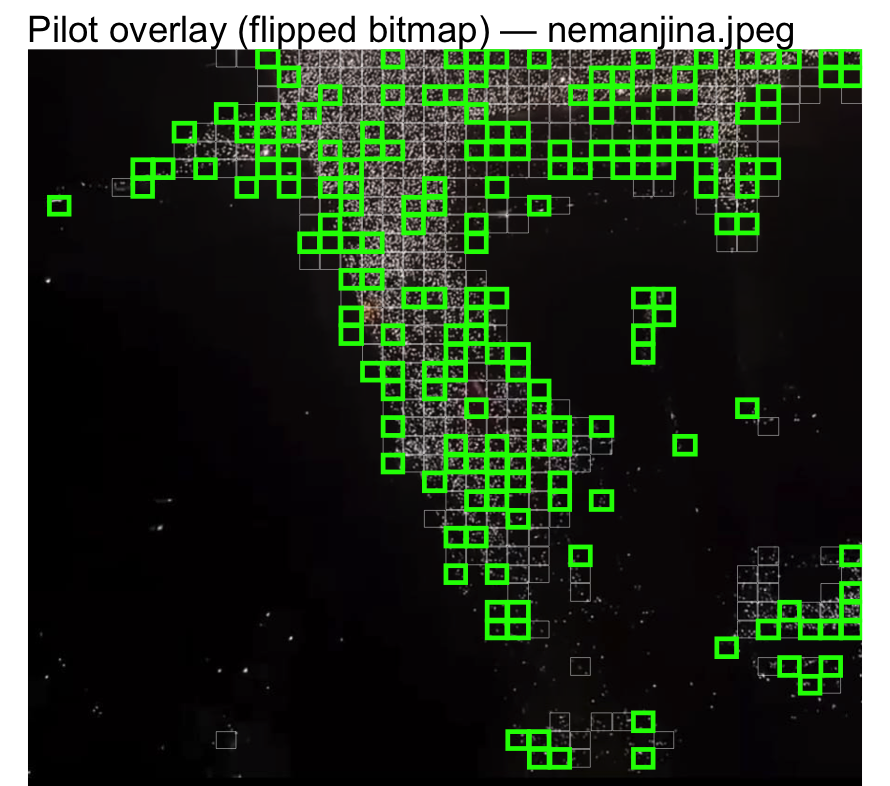
\includegraphics[width=\textwidth]{../outputs/sampling_outputs/main_overlays_image/main_overlay_nemanjina.png}
	  \caption{Nemanjina}
	  \label{fig:nemanjina}
	\end{subfigure}
	\hfill
	\begin{subfigure}[b]{0.3\textwidth}
		\centering
		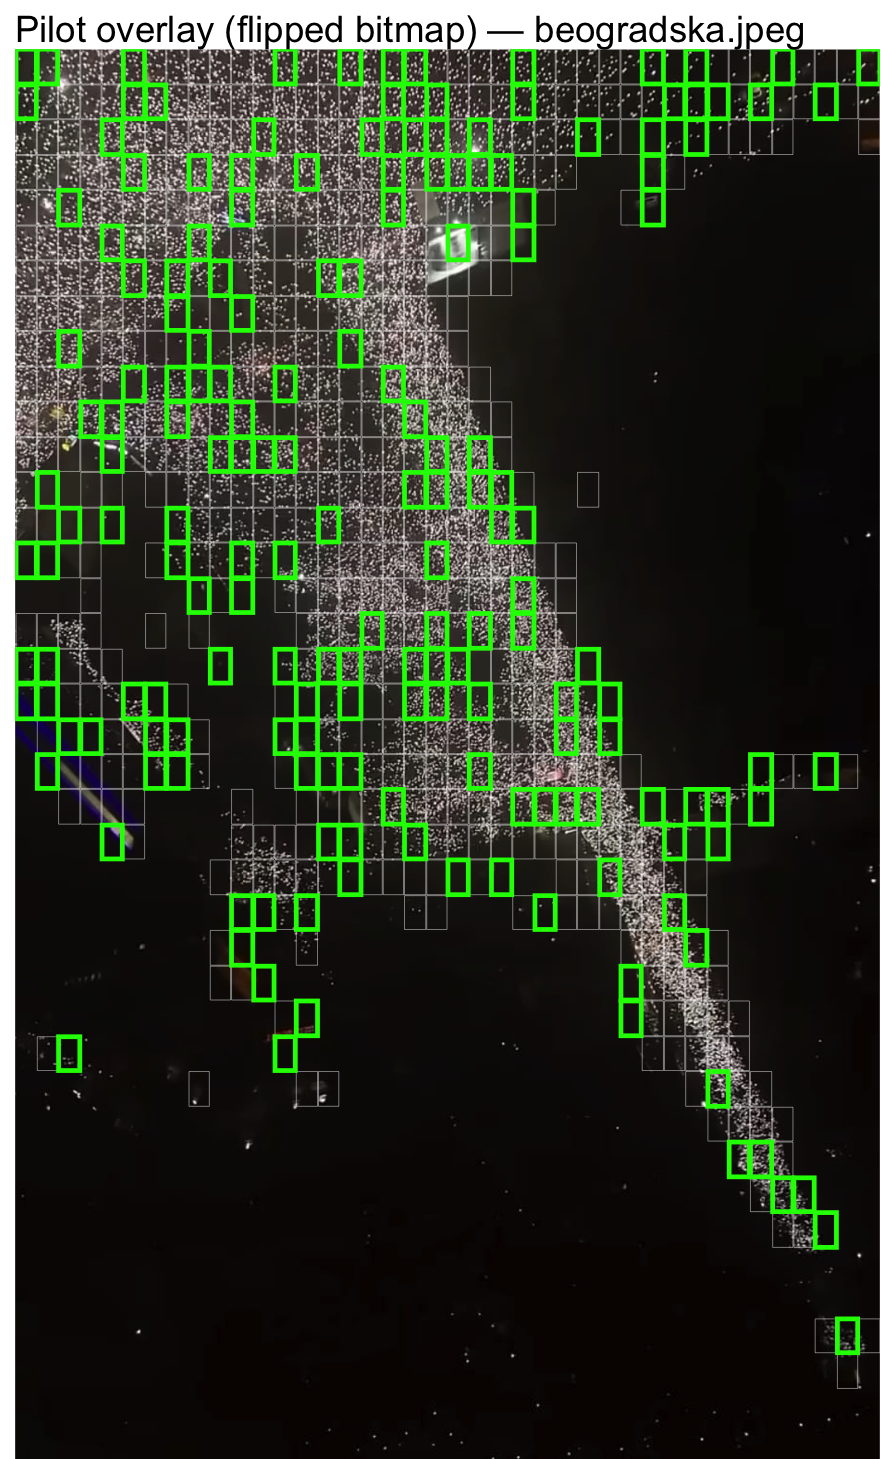
\includegraphics[width=\textwidth]{../outputs/sampling_outputs/main_overlays_image/main_overlay_beogradska.png}
		\caption{Beogradska}
		\label{fig:beogradska}
	\end{subfigure}
  
	\vspace{0.3cm} % razmak između redova
  
	% Drugi red
	\begin{subfigure}[b]{0.3\textwidth}
	  \centering
	  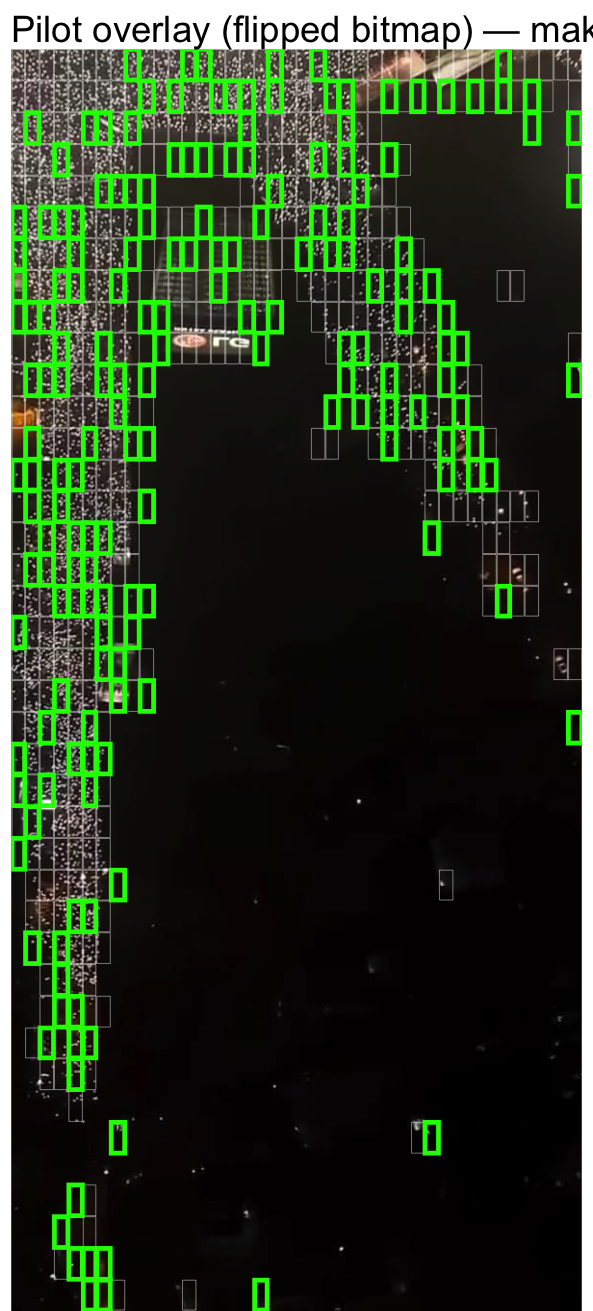
\includegraphics[width=\textwidth]{../outputs/sampling_outputs/main_overlays_image/main_overlay_makenzijeva.png}
	  \caption{Makenzijeva}
	  \label{fig:makenzijeva}
	\end{subfigure}
	\hfill
	\begin{subfigure}[b]{0.3\textwidth}
	  \centering
	  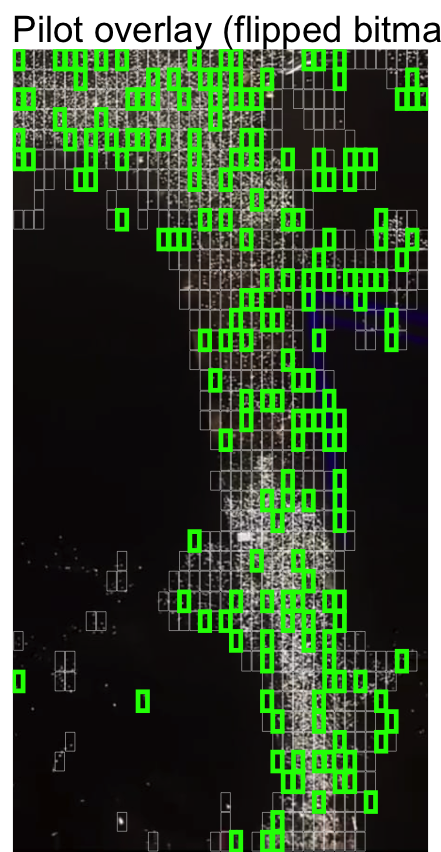
\includegraphics[width=\textwidth]{../outputs/sampling_outputs/main_overlays_image/main_overlay_kralja-milana.png}
	  \caption{Kralja Milana}
	  \label{fig:kralja-milana}
	\end{subfigure}
	\hfill
	\begin{subfigure}[b]{0.3\textwidth}
	  \centering
	  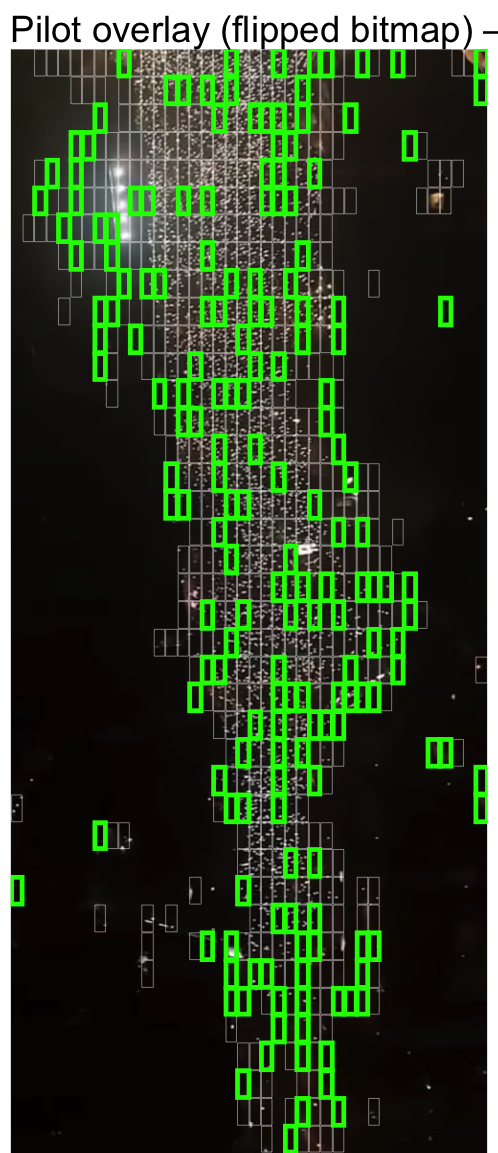
\includegraphics[width=\textwidth]{../outputs/sampling_outputs/main_overlays_image/main_overlay_bulevar-oslobodjenja.png}
	  \caption{Bulevar oslobođenja}
	  \label{fig:bulevar-oslobodjenja}
	\end{subfigure}
  
	\caption{Prikaz preklopa (overlay) ćelija za glavno uzorkovanje preko svake slike}
\end{figure}

\noindent
Ovaj vizuelni prikaz će nam omogućiti da lakše odredimo u kojim ćelijamo brojimo bliceve. 
Kako bismo popunili napravljeni CSV, koristićemo automatsko brojanje bliceva pomoću python skripte \texttt{auto-count.py}, o kojoj će biti više
reči u nastavku. Dodatno za neke ćelije koristili smo ručno brojanje.


\subsection{Automatsko brojanje (Python)}

Koristimo skriptu (auto-count.py) koja popunjava kolonu y u \texttt{pilot\_to\_count.csv} ili \texttt{main\_to\_count.csv}.
\newline
\noindent Ulaz: 
\begin{itemize}
	\item \texttt{frame\_csv} = \texttt{strata\_map\_auto.csv} (sve ćelije sa koordinatama).
	\item \texttt{pilot\_csv} ili \texttt{main\_csv} (lista ciljnih ćelija za brojanje: \texttt{img\_path}, stratum, \texttt{cell\_id}, y).
\end{itemize}
\noindent Izlaz:
\begin{itemize}
	\item CSV sa popunjenim y
	\item Per-image „clean count“ pregled (cela slika sa označenim pilot/main ćelijama i svim detektovanim tačkama).
\end{itemize}

\begin{figure}[H] 
	\centering 
	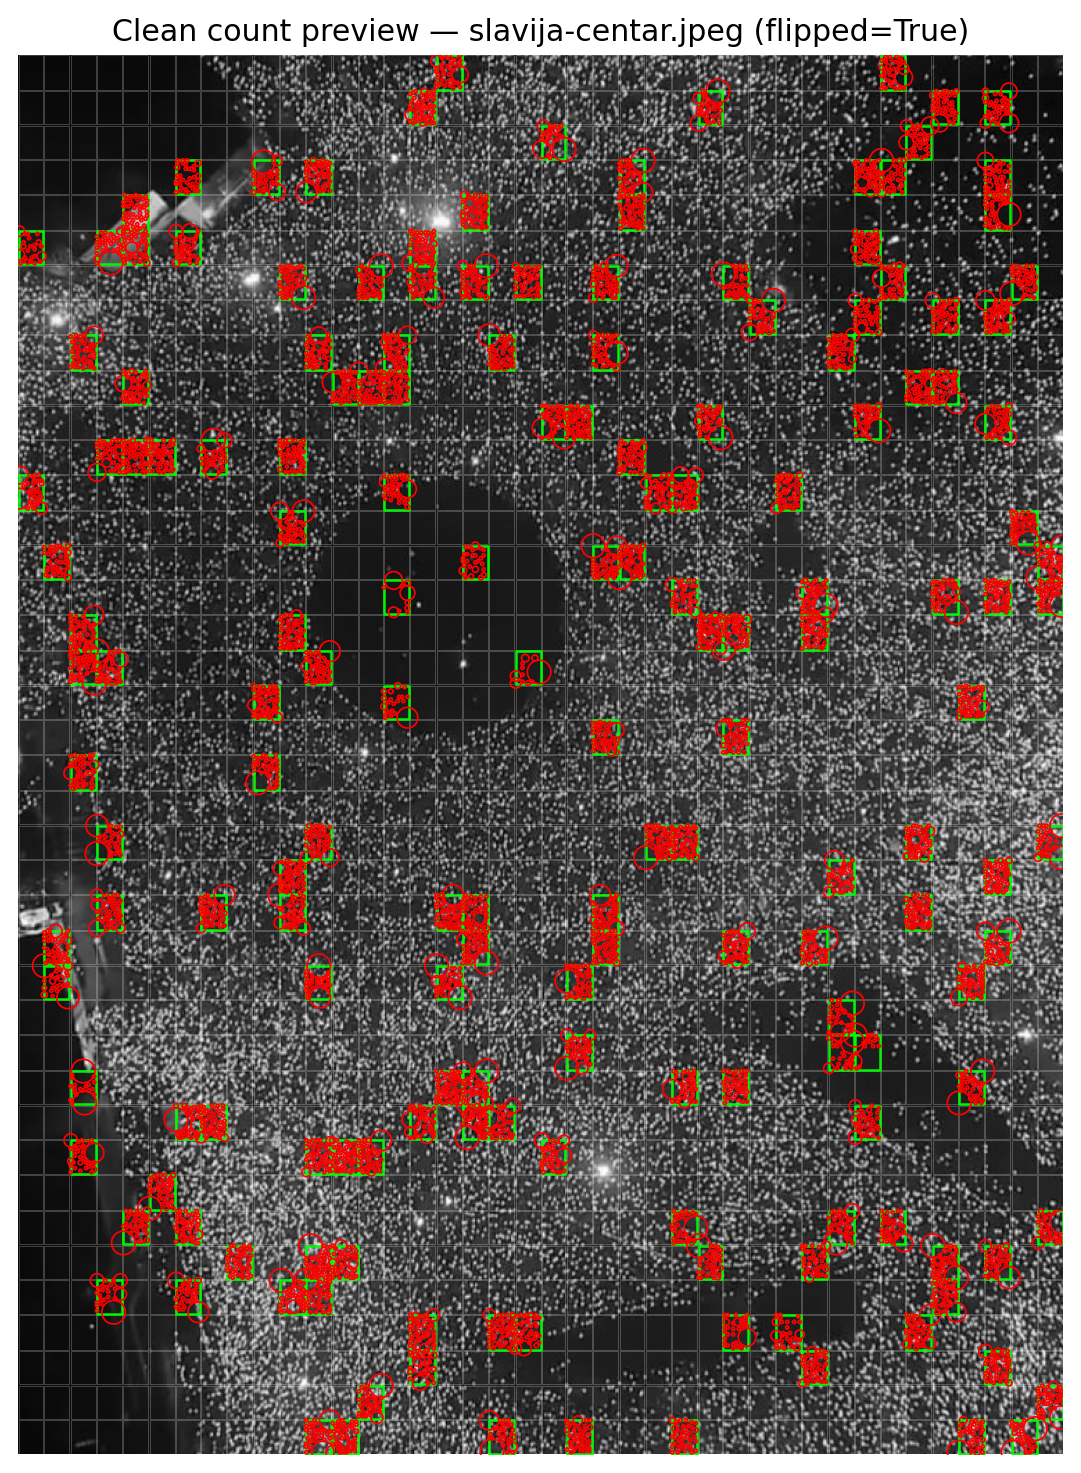
\includegraphics[width=0.8\textwidth]{../outputs/sampling_outputs/previews_images_main/slavija-centar_pilot_clean_count_preview.png} 
	\caption{Slavija.} 
	\label{fig:slavija} 
\end{figure}

\begin{figure}[H]
	\centering
  
	% Prvi red
	\begin{subfigure}[b]{0.3\textwidth}
	  \centering
	  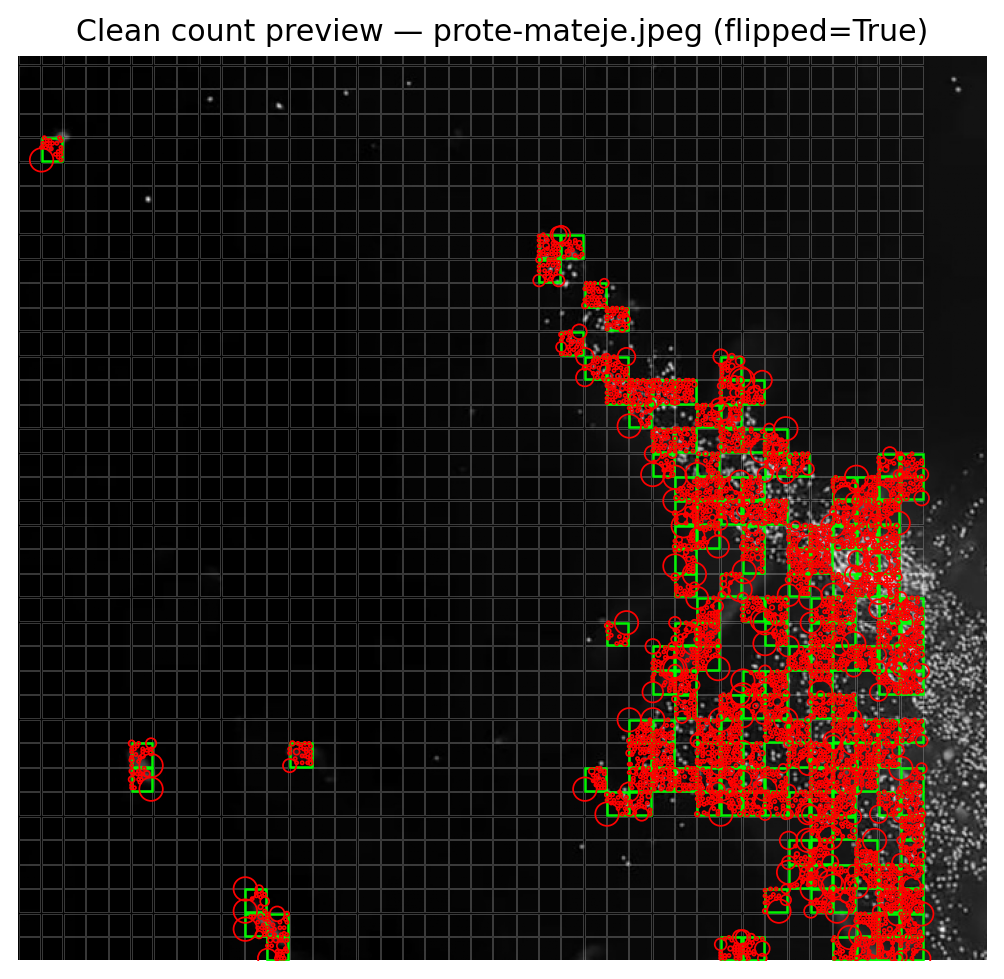
\includegraphics[width=\textwidth]{../outputs/sampling_outputs/previews_images_main/prote-mateje_pilot_clean_count_preview.png}
	  \caption{Prote Mateje}
	  \label{fig:prote-mateje}
	\end{subfigure}
	\hfill
	\begin{subfigure}[b]{0.3\textwidth}
	  \centering
	  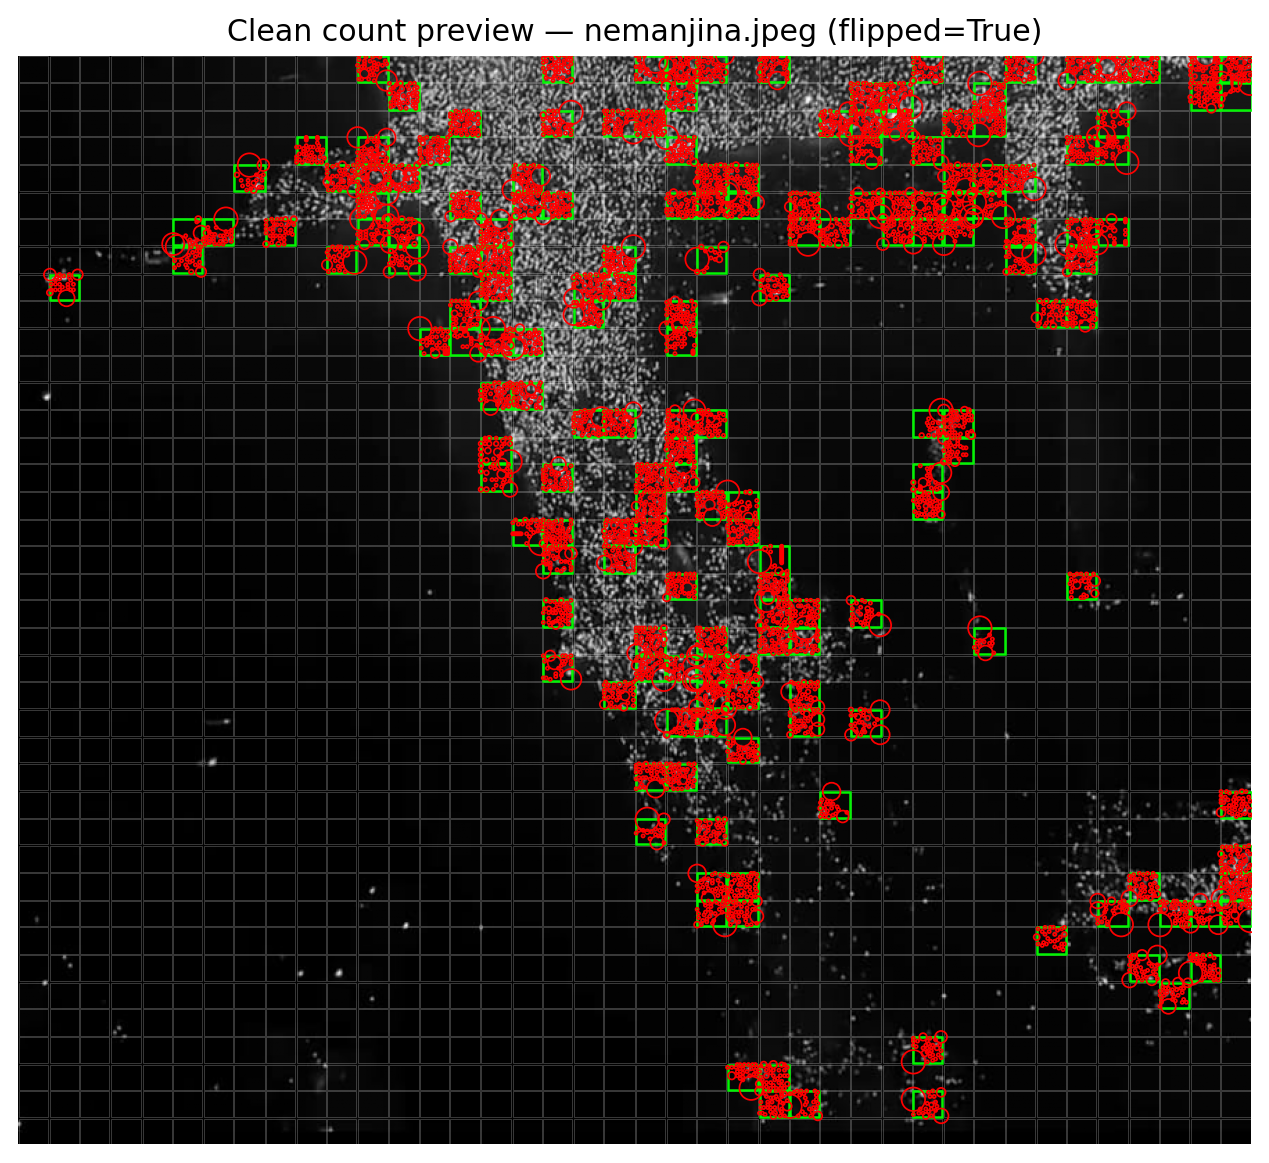
\includegraphics[width=\textwidth]{../outputs/sampling_outputs/previews_images_main/nemanjina_pilot_clean_count_preview.png}
	  \caption{Nemanjina}
	  \label{fig:nemanjina}
	\end{subfigure}
	\hfill
	\begin{subfigure}[b]{0.3\textwidth}
		\centering
		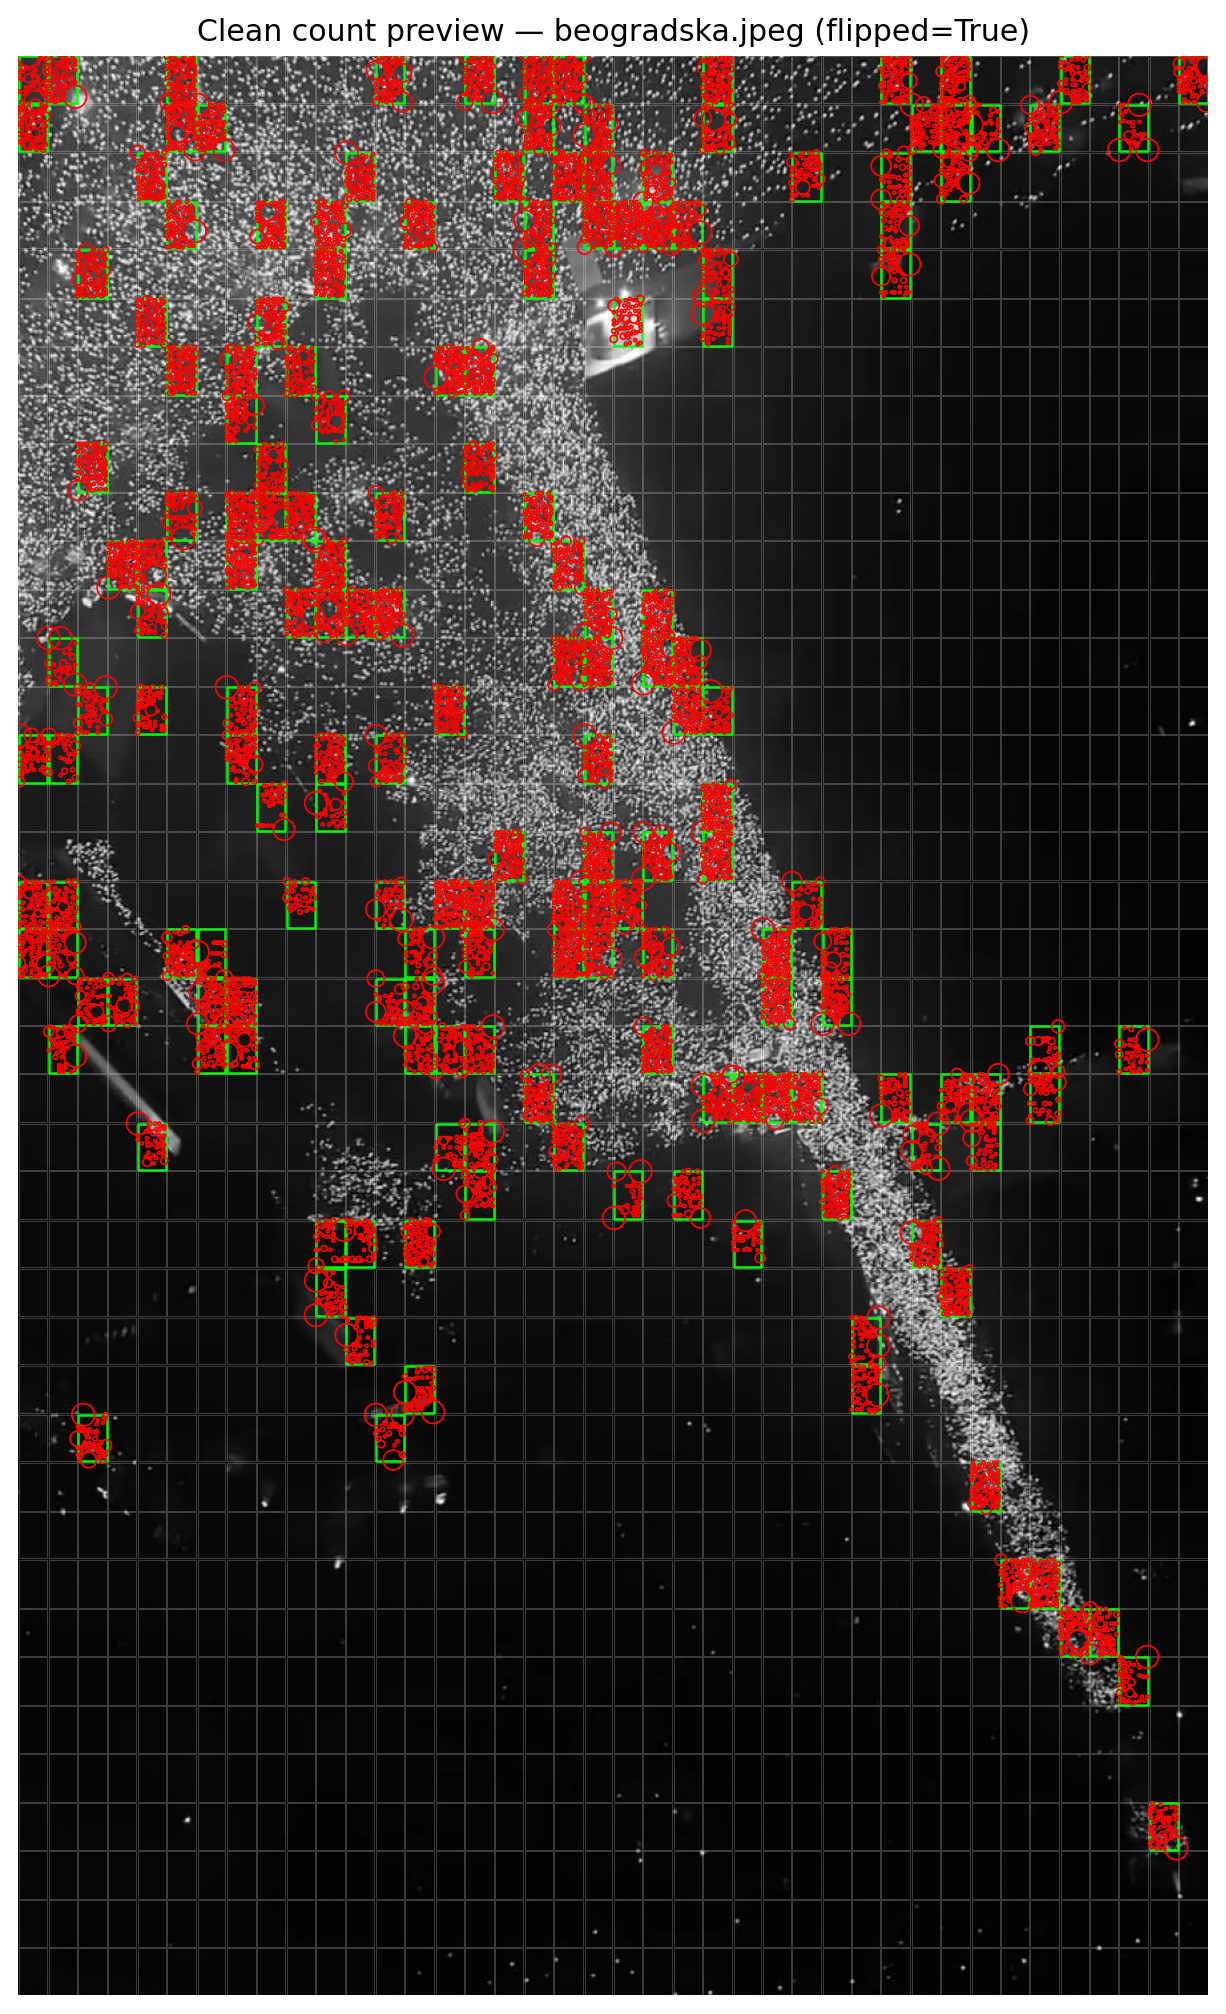
\includegraphics[width=\textwidth]{../outputs/sampling_outputs/previews_images_main/beogradska_pilot_clean_count_preview.png}
		\caption{Beogradska}
		\label{fig:beogradska}
	\end{subfigure}
  
	\vspace{0.3cm} % razmak između redova
  
	% Drugi red
	\begin{subfigure}[b]{0.3\textwidth}
	  \centering
	  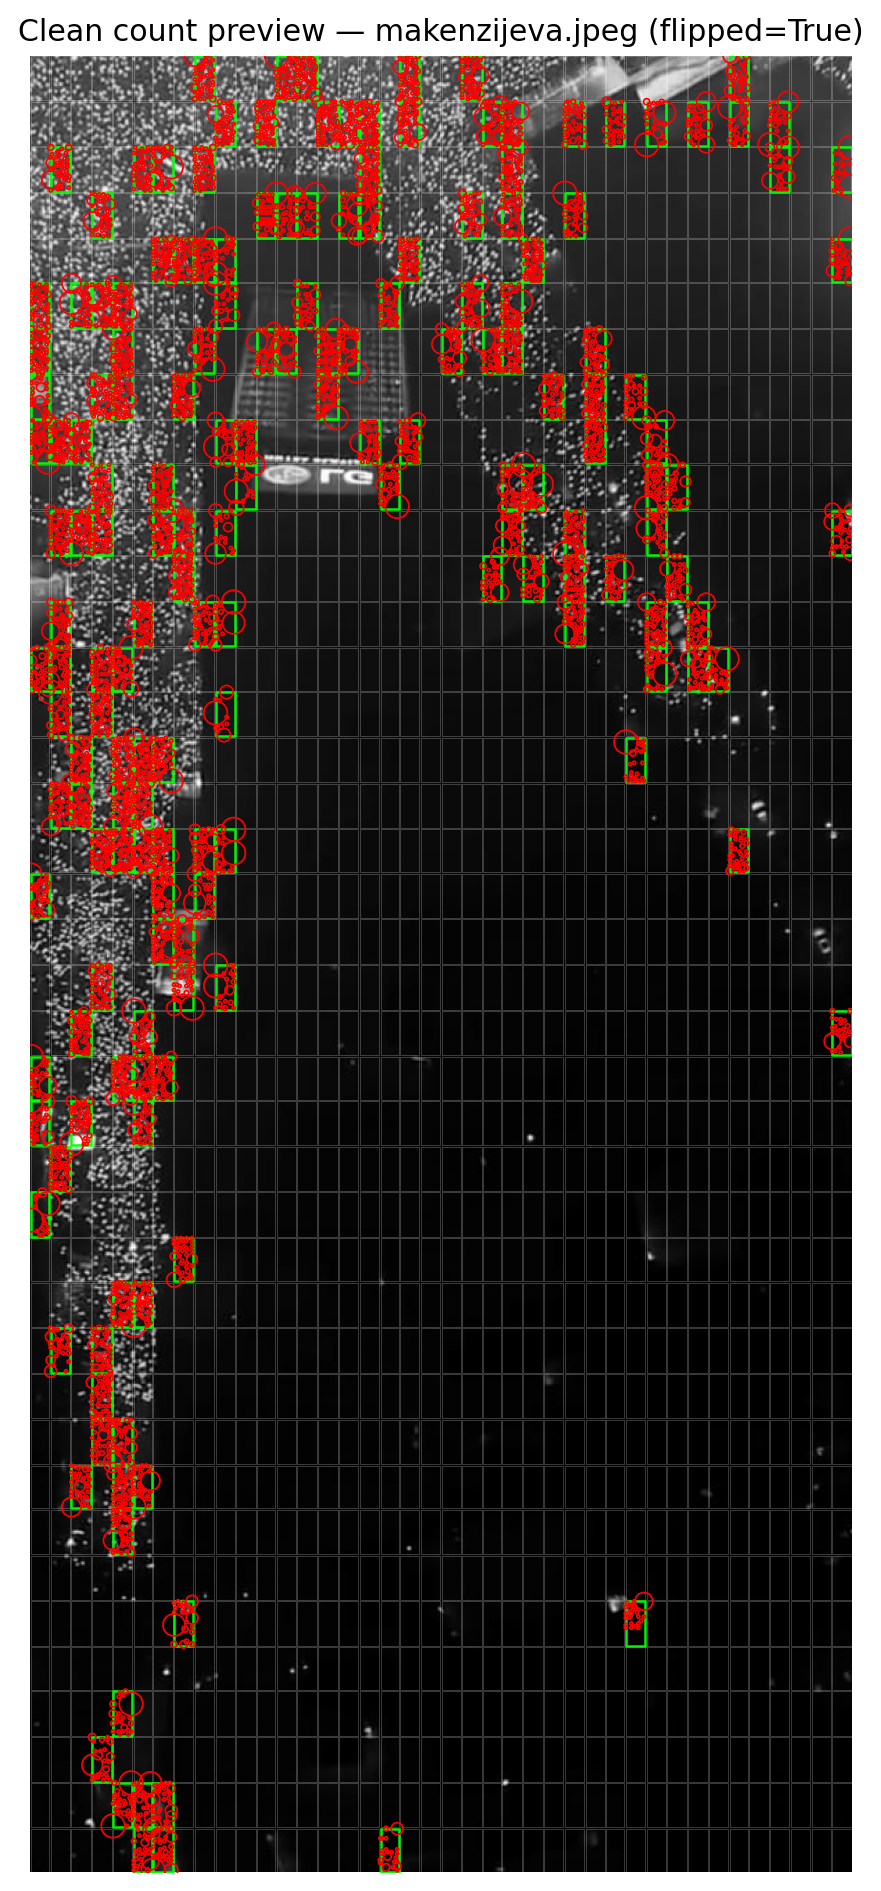
\includegraphics[width=\textwidth]{../outputs/sampling_outputs/previews_images_main/makenzijeva_pilot_clean_count_preview.png}
	  \caption{Makenzijeva}
	  \label{fig:makenzijeva}
	\end{subfigure}
	\hfill
	\begin{subfigure}[b]{0.3\textwidth}
	  \centering
	  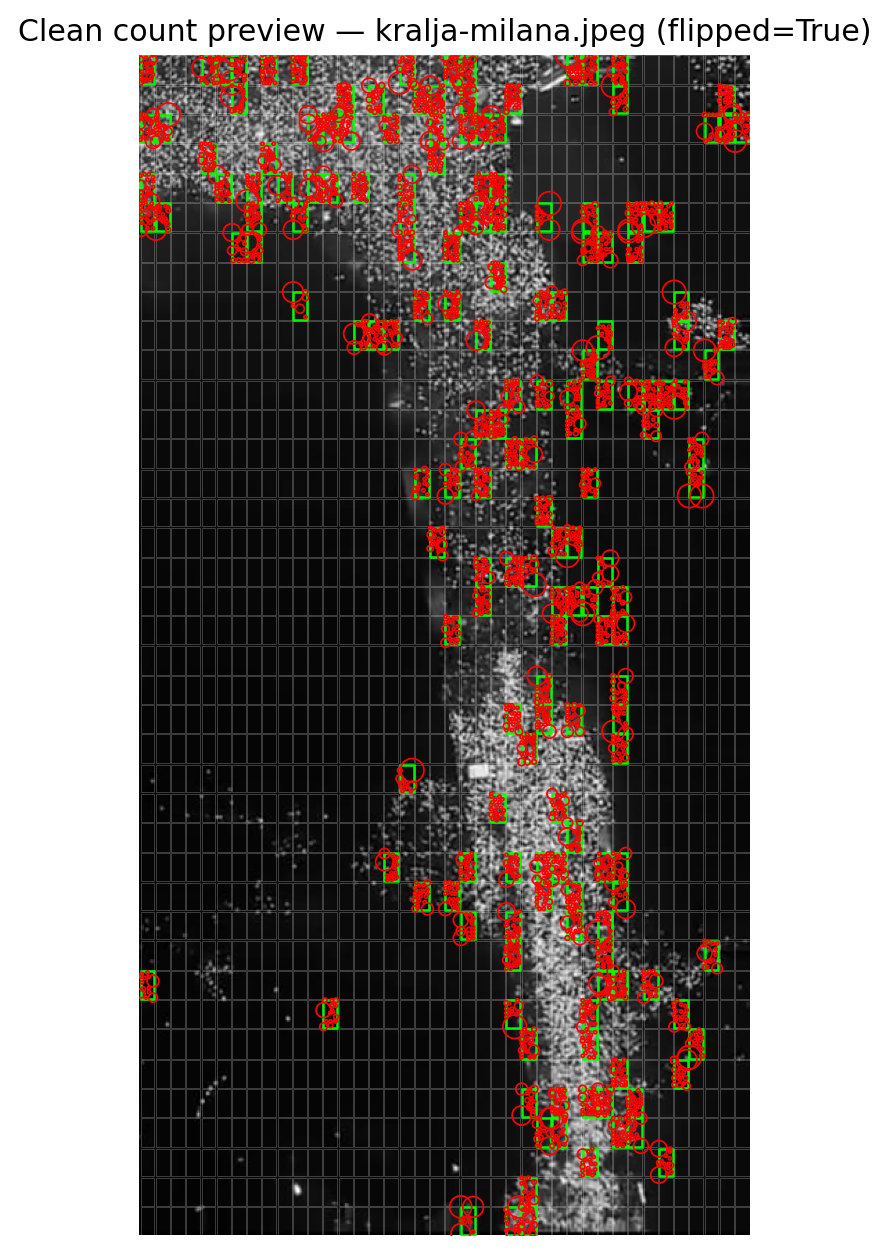
\includegraphics[width=\textwidth]{../outputs/sampling_outputs/previews_images_main/kralja-milana_pilot_clean_count_preview.png}
	  \caption{Kralja Milana}
	  \label{fig:kralja-milana}
	\end{subfigure}
	\hfill
	\begin{subfigure}[b]{0.3\textwidth}
	  \centering
	  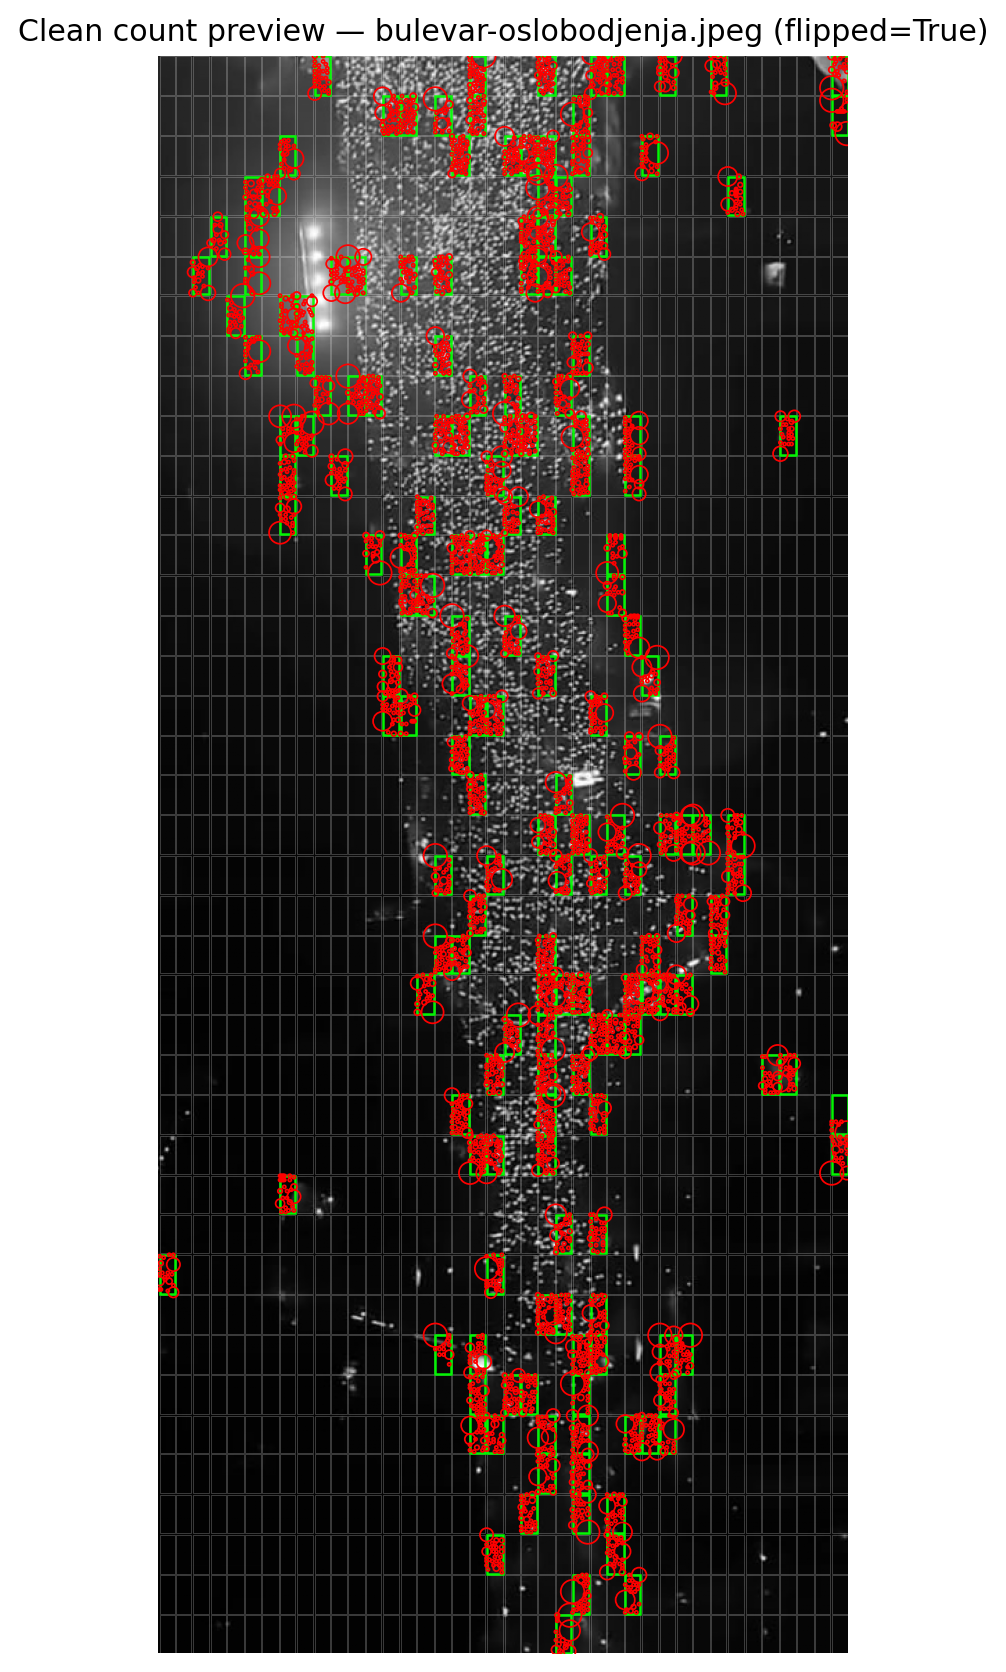
\includegraphics[width=\textwidth]{../outputs/sampling_outputs/previews_images_main/bulevar-oslobodjenja_pilot_clean_count_preview.png}
	  \caption{Bulevar oslobođenja}
	  \label{fig:bulevar-oslobodjenja}
	\end{subfigure}
  
	\caption{Per-image „clean count“ pregled za glavno uzorkovanje}
\end{figure}


\noindent
Detekcija (pipeline):
\begin{enumerate}
  \item \textbf{CLAHE:} pojačavanje lokalnog kontrasta - pojačava sitne detalje i smanjuje uticaj globalnog osvetljenja.
  \item \textbf{White tophat:} uklanjanje širokih oreola/sjaja, ostavljajući sitne tačkice.
  \item \textbf{Maska „vrućih“ regiona:} (Gaussian + prag + blago širenje) - spreči lažno detektovanje po jakim odsjajima.
  \item \textbf{LoG (Laplacian of Gaussian):} traži “kružne” sitne strukture sa ograničenjem skale
\end{enumerate}

\section{Ocene i intervali poverenja}

Neka su $h=1,2,3$ stratumi, $N_h$ broj dostupnih ćelija u stratumu $h$ (u okviru jedne slike), a $n_h$ broj uzorkovanih ćelija u istom stratumu. 
Za svaku izabranu ćeliju merimo $y$ (broj ``tačkica''/detekcija u ćeliji). Pretpostavka je da su posmatranja unutar stratuma prost slučajni uzorak bez ponavljanja; slike su međusobno disjunktne (bez preklapanja).
\newline
\newline
\noindent
Za jednu sliku, stratumsku sredinu ocenjujemo kao
\[
\bar y_h \;=\; \frac{1}{n_h}\sum_{i=1}^{n_h} y_{hi}, 
\qquad
s_h^2 \;=\; \frac{1}{n_h-1}\sum_{i=1}^{n_h}\bigl(y_{hi}-\bar y_h\bigr)^2,
\]
uz konvenciju $s_h^2=0$ kada je $n_h=1$.
Ukupan broj (total) za sliku ocenjujemo:
\[
\hat T \;=\; \sum_{h=1}^H N_h\,\bar y_h.
\]
Ocenu varijanse dobijamo sa korekcijom konačne populacije po stratumu:
\[
\widehat{\mathrm{Var}}(\hat T) \;=\; \sum_{h=1}^H 
N_h^2 \left(1-\frac{n_h}{N_h}\right)\frac{s_h^2}{n_h}.
\]
Standardna greška je $\mathrm{SE}=\sqrt{\widehat{\mathrm{Var}}(\hat T)}$, a za nivo poverenja $1-\alpha$ koristimo
\[
\hat T \;\pm\; z_{1-\alpha/2}\cdot \mathrm{SE},
\]
gde je $z_{1-\alpha/2}$ kvantil standardne normalne raspodele (u praksi $\alpha=0{.}05$, pa je $z_{0{.}975}\approx 1{.}96$).

\paragraph{Napomena o malim uzorcima.}
Ako su $n_h$ vrlo mali (npr.\ $n_h\le 5$), interval poverenja zasnovan na $t$-kvantilu sa $n_h-1$ stepeni slobode može biti konzervativniji; u ovom radu, imajući u vidu veličine uzoraka po stratumu, z-kvantili su adekvatni.
\newline
\newline
\noindent
Kako su slike disjunktne, ukupna ocena za ceo skup dobija se sabiranjem po slikama:
\[
\hat T_{\mathrm{tot}} \;=\; \sum_{j} \hat T_j,
\qquad
\widehat{\mathrm{Var}}(\hat T_{\mathrm{tot}}) \;=\; \sum_{j} \widehat{\mathrm{Var}}(\hat T_j),
\]
pa je $\mathrm{SE}_{\mathrm{tot}}=\sqrt{\sum_j \widehat{\mathrm{Var}}(\hat T_j)}$ i interval poverenja glasi
\[
\hat T_{\mathrm{tot}} \;\pm\; z_{1-\alpha/2}\cdot \mathrm{SE}_{\mathrm{tot}}.
\]

\newpage
\section{Rezultati i diskusija}

Kad se popravi ono, promeni brojeve 
\newline
\noindent
U Tabeli \ref{tab:results} prikazani su rezultati, odnosno ocene dobijene po pojedinačnim slikama, kao i ukupna ocena.

\begin{table}[H]
\centering
\begin{tabular}{lrrrr}
\hline
Slika & $\hat T$ & SE & CI donja & CI gornja \\
\hline
\texttt{beogradska.jpeg}          & 41,056  & 383 & 40,306  & 41,807  \\
\texttt{bulevar-oslobodjenja.jpeg}& 17,339  & 213 & 16,922  & 17,756  \\
\texttt{kralja-milana.jpeg}       & 13,815  & 182 & 13,459  & 14,171  \\
\texttt{makenzijeva.jpeg}         & 19,767  & 215 & 19,345  & 20,188  \\
\texttt{nemanjina.jpeg}           & 15,405  & 175 & 15,062  & 15,748  \\
\texttt{prote-mateje.jpeg}        & 5,544   & 48  & 5,451   & 5,637   \\
\texttt{slavija-centar.jpeg}      & 57,479  & 703 & 56,100  & 58,857  \\
\hline
\textbf{Ukupno}                   & \textbf{170,405} & \textbf{894} & \textbf{168,653} & \textbf{172,156} \\
\hline
\end{tabular}
\caption{Procene ukupnog broja bliceva po slici i ukupno, sa 95\% intervalima poverenja.}
\label{tab:results}
\end{table}

Dobijeni rezultati ukazuju da je ukupna procena broja ljudi na osnovu registrovanih bliceva na posmatranim lokacijama iznosila približno 170.405, uz standardnu grešku od 894 i 95\% interval poverenja $[168.653, 172.156]$. Vidimo da najveći doprinos ukupnoj proceni daje područje Slavije (oko 57.470 ljudi) i ulice Beogradske (oko 41.056 ljudi), što je i očekivano s obzirom na prostorni raspored i gustinu okupljenih. Ostale lokacije, poput Nemanjine ili Makenzijeve, imale su značajno manji, ali ne zanemarljiv doprinos, dok su ulice poput Prote Mateje imale vrlo mali broj učesnika u poređenju sa centralnim čvorištima.

\newpage
\section{Zaključak}
Na protestu održanom 15. marta 2025. godine u Beogradu, prema proceni Arhiva javnih skupova, prisustvovalo je između 275.000 i 325.000 ljudi, uz mogućnost da je taj broj bio i veći. \cite{n1protest15za15}
. Ovaj skup je bio jedan od najvećih u novijoj istoriji Srbije, nadmašujući prethodne proteste po broju učesnika. Međutim, Ministarstvo unutrašnjih poslova Republike Srbije je procenilo da je broj učesnika bio oko 107.000 \cite{insajder_mup_15za15}, što je značajno niže od nezavisnih procena.

Razlike u procenama broja učesnika mogu biti posledica različitih metodoloških pristupa, političkih stavova i ciljeva. Razlike ukazuju i na važnost transparentne metodologije i jasno definisanih kriterijuma brojanja.

U okviru ovog rada, sproveli smo vlastito brojanje učesnika, pri čemu je zabeležen rezultat od oko 170.000 ljudi. Važno je napomenuti da je ovo brojanje izvedeno samo na osnovu prisustva upaljenih „bliceva“ i isključivo u okolini Slavije, dok su procene Arhiva i MUP-a obuhvatale dosta šire teritorije grada i dodatne lokacije gde su se učesnici okupljali. Stoga se naš rezultat ne može direktno porediti sa ukupnim procenama, ali pruža uvid u lokalnu gustinu učesnika i omogućava uporedivu kvantifikaciju na odabranoj lokaciji.
\newpage
\begin{thebibliography}{9}

	\bibitem{drone_video}
	Autor nepoznat. 
	\textit{Snimak javnog okupljanja dronom}. 
	Dostupno na: \url{https://youtube.com/shorts/4pbj2aZAoP4?si=wxzp9pIkflD2CYKN} 
	(Pristupljeno: 25. septembar 2025.)
	
	\bibitem{n1protest15za15}
	N1 Beograd,
	\emph{Arhiv javnih skupova izneo procenu o broju učesnika na protestu „15. za 15“},
	15. mart 2025,
	\url{https://n1info.rs/vesti/arhiv-javnih-skupova-izneo-procenu-o-broju-ucesnika-na-protestu-15-za-15/}.

	\bibitem{insajder_mup_15za15}
	Insajder,
	\emph{MUP o skupu „15. za 15“: U piku na svim lokacijama oko 107.000 ljudi},
	15. mart 2025,
	\url{https://www.insajder.net/prenosimo/mup-o-skupu-15-za-15-u-piku-na-svim-lokacijama-oko-107000-ljudi}.

	\end{thebibliography}

\end{document}